\documentclass{ieeeaccess}
\usepackage{cite}
\usepackage{amsmath,amssymb,amsfonts}
\usepackage{algorithmic}
\usepackage{graphicx}
\usepackage{textcomp}
\usepackage{bm}
\makeatletter
\AtBeginDocument{\DeclareMathVersion{bold}
\SetSymbolFont{operators}{bold}{T1}{times}{b}{n}
\SetSymbolFont{NewLetters}{bold}{T1}{times}{b}{it}
\SetMathAlphabet{\mathrm}{bold}{T1}{times}{b}{n}
\SetMathAlphabet{\mathit}{bold}{T1}{times}{b}{it}
\SetMathAlphabet{\mathbf}{bold}{T1}{times}{b}{n}
\SetMathAlphabet{\mathtt}{bold}{OT1}{pcr}{b}{n}
\SetSymbolFont{symbols}{bold}{OMS}{cmsy}{b}{n}
\renewcommand\boldmath{\@nomath\boldmath\mathversion{bold}}
% ieeeaccess.cls captions use \mathversion{medium} but leave letters/symbols
% unset for medium (and regular/black), so \Delta in \caption renders as U+00B4.
% ieeeaccess.cls maps uppercase Greek (\Delta etc.) to operators slots 00--0A.
% Formata (T1) has no Greek there (acute shows instead); CMR does.
\SetSymbolFont{operators}{regular}{OT1}{cmr}{m}{n}
\SetSymbolFont{operators}{medium}{OT1}{cmr}{m}{n}
\SetSymbolFont{operators}{black}{OT1}{cmr}{m}{n}
\SetSymbolFont{letters}{regular}{OML}{cmm}{m}{it}
\SetSymbolFont{letters}{medium}{OML}{cmm}{m}{it}
\SetSymbolFont{letters}{black}{OML}{cmm}{m}{it}
\SetSymbolFont{letters}{bold}{OML}{cmm}{b}{it}
\SetSymbolFont{symbols}{regular}{OMS}{cmsy}{m}{n}
\SetSymbolFont{symbols}{medium}{OMS}{cmsy}{m}{n}
\SetSymbolFont{symbols}{black}{OMS}{cmsy}{m}{n}
\SetSymbolFont{largesymbols}{regular}{OMX}{cmex}{m}{n}
\SetSymbolFont{largesymbols}{medium}{OMX}{cmex}{m}{n}
\SetSymbolFont{largesymbols}{black}{OMX}{cmex}{m}{n}
\SetSymbolFont{largesymbols}{bold}{OMX}{cmex}{b}{n}
% Keep caption text in Formata; math inherits CMR operators (Greek-safe).
\renewcommand\figcapfont{\def\textit##1{{\sffamily\fontshape{it}\selectfont##1}}\sffamily\fontencoding{T1}\fontfamily{formata}\fontseries{m}\fontsize{7}{8.4}\selectfont\regularmath}
\renewcommand\tablecapfont{\def\textit##1{{\sffamily\fontshape{it}\selectfont##1}}\sffamily\fontencoding{T1}\fontfamily{formata}\fontseries{m}\fontsize{7}{8.4}\selectfont\regularmath}
}
\makeatother

\def\BibTeX{{\rm B\kern-.05em{\sc i\kern-.025em b}\kern-.08em
    T\kern-.1667em\lower.7ex\hbox{E}\kern-.125emX}}

\begin{document}
\history{Date of publication xxxx 00, 0000, date of current version xxxx 00, 0000.}
\doi{10.1109/ACCESS.2024.0429000}

\title{Resource Frames, Graph Scope, and Rail States: Conditional Decision Boundaries for Reserve-Force Bus versus Rail--Bus Multimodal Transport}

\author{\uppercase{Hyunjun Kim}\authorrefmark{1,2},
\uppercase{Jae Woo Lee}\authorrefmark{1,3}, AND \uppercase{Hyunho Kim}\authorrefmark{1}}

\address[1]{Korea Military Academy, Seoul 01805, Republic of Korea (e-mail: kimhyuh@kma.ac.kr)}
\address[2]{Korea Advanced Institute of Science and Technology (KAIST), Daejeon, Republic of Korea (e-mail: hyunjun1121@kaist.ac.kr)}
\address[3]{CHA University, Seongnam, Republic of Korea (e-mail: simonlee98@chauniv.ac.kr)}

\markboth
{H. Kim et al.: Conditional Decision Boundaries for Reserve-Force Transport}
{H. Kim et al.: Conditional Decision Boundaries for Reserve-Force Transport}

\corresp{Corresponding author: Hyunho Kim (e-mail: kimhyuh@kma.ac.kr).}

\begin{abstract}
Wartime reserve-force transport planning often compares bus-only road movement with rail--bus multimodal movement under disrupted links, yet a modal ranking is uninterpretable unless the resource frame, reduced-graph scope, rail availability state, fleet allocation, and response rule are stated explicitly. This article reports a public-data-based conditional scenario simulation on a Songpa--Goseong case corridor using the Korean Standard Node-Link road network. Top-10 corridor graphs (9{,}089 nodes; 18{,}602 edges) are audited against a full reference graph (360{,}556 nodes; 971{,}680 edges); road vehicles complete passenger travel, traverse the reverse road network empty, and incur turnaround before reuse; rail is represented by available, degraded, and unavailable service states. Fifteen campaign sets produced 29{,}940 runs under common-random-number seed blocks with paired $t$ intervals, 10{,}000-replicate percentile bootstrap intervals, a joint-seed break-even bootstrap, a crossed two-way random-threat bootstrap, and Morris elementary-effect screening on completion rate. Under configured resource bundles (23 direct road vehicles versus 46 road vehicles plus rail), mean completion times are 374.1 and 363.8 min and the paired difference includes zero. Under an equal total road fleet of 23 vehicles, the comparison is allocation-conditional: sweeping all 23 feasible feeder/last-mile splits shows a U-shaped surface whose best split (6 feeder + 17 last-mile, 394.6 min) leaves bus-only statistically tied ($-20.5$ min, intervals include zero), while the arbitrary fixed 12/11 split (475.8 min) inflates the bus advantage to $-101.7$ min. The long-haul road-damage break-even is therefore a band, not a point: robust splits cross near 1.150--1.277, the fixed 12/11 split at 1.742 (joint-seed interval 1.550--2.003). Full-graph validation reproduces both crossings (1.761 and 1.150 with matching intervals), and a second corridor (Songpa--Yangyang) reproduces the protocol diagnostics with different numbers (audit pattern identical, crossing 1.278 at its own best split). Top-5 and top-10 graphs match full-scope connectivity and policy ranking in the tested conditions, whereas top-3 does not. When rail is unavailable, static multimodal transport does not complete, while a precheck switching policy ties bus-only. The contribution is a conditional decision boundary and a reporting protocol for resource frames and graph scope, not a general claim that either mode is superior.
\end{abstract}

\begin{keywords}
Break-even analysis, common random numbers, discrete-event simulation, multimodal transport, network reduction, reserve-force transport.
\end{keywords}

\titlepgskip=-21pt

\maketitle

\section{Introduction}
\label{sec:introduction}
\PARstart{R}{eserve-force} mobilization transport must move large person batches from assembly zones to destination areas under wartime disruption, limited road fleets, and uncertain rail service. Decision makers frequently frame the problem as bus-only versus rail--bus multimodal comparison. Simulation studies of wartime multimodal movement show that terrain-aware speeds, transfer stages, and finite fleets can reverse naive capacity rankings \cite{b1}. Network vulnerability research further shows that link closure costs depend on exposure and rerouting structure rather than on a single criticality score alone \cite{b10,b19}. Yet published comparisons rarely separate three design choices that jointly determine the reported winner: (i) how road and rail resources are counted, (ii) whether the analysis graph is a reduced corridor envelope or the full national network, and (iii) whether rail is available, degraded, or unavailable as an explicit service state.

This article develops conditional decision boundaries for a public-data Songpa--Goseong case corridor over a 24-h (1{,}440 min) window with approximately 1{,}000 mobilized reservists. Two alternatives share the same disruption scenarios and common-random-number (CRN) seed block: \emph{bus-only} moves assembly~A to destination~D by road; \emph{static multimodal} moves A to rail access~S by feeder shuttle, S to rail egress~R by chartered nonstop rail, then R to D by last-mile bus. Coordinates are public administrative centroids and public rail stations only; no unit facility location, order of battle, or movement schedule is modeled. The practical motivation is narrow and explicit: reserve-force mobilization planners who compare bus and rail--bus options under wartime disruption need to know whether an observed modal ranking survives a change in how vehicles are counted, how much of the national graph is kept, whether rail is treated as a service state, and whether the response policy is allowed to adapt.

The study asks six questions. First, how well do top-3, top-5, and top-10 corridor graphs preserve full-graph connectivity, normal travel time, and bus-versus-multimodal ranking under shared stress conditions? Second, how does the no-disruption comparison change between a configured resource-bundle frame and an equal-total-road-fleet frame? Third, with normally available rail in the equal-road-fleet frame, at what long-haul road slowdown does the mean completion-time ordering cross, and how stable is that crossing under a finer multiplier grid? Fourth, how do rail degradation, rail unavailability, random threat locations, fleet scarcity, demand scale, and adaptive response policies alter the comparison? Fifth, what do physical empty-return and vehicle-cycle KPIs reveal that passenger makespan alone hides? Sixth, under budget-$k$ path interdiction on the reduced corridor envelope, does the comparison complete at all, and how should such a result be scoped?

Six methodological contributions organize the experiments. (1) Graph scope is audited against a full reference graph rather than justified only by normal shortest-path time, using connectivity agreement, policy-ranking agreement, and functional-segment normal-time ratios as three separate diagnostics. (2) Vehicle reuse requires a physical empty return over the current reverse road network plus turnaround; empty-return trips, empty-return minutes, and road-vehicle cycles are first-class KPIs. (3) Configured bundles and equal-total-road-fleet comparisons are reported separately; the latter still includes rail and is not an equal-cost comparison. (4) Paired $t$ intervals, percentile bootstrap intervals, joint-seed break-even uncertainty, two-level threat/arrival uncertainty, and Morris elementary effects on completion rate are reported as distinct inference products, with replicate-count half-width sequences that prevent a blanket claim that thirty runs are universally adequate. (5) Results are stated as conditional decision boundaries and response-policy rankings rather than a single modal ranking. (6) Adversarial path interdiction is reported as a graph-scope-sensitive stress product that does not enter the break-even estimate, because zero-completion cells on a reduced envelope are not full-network proofs.

The argument chain of the article is deliberate: resource frame and graph scope are fixed before any disruption claim (Sections~III--V); paired CRN differences are estimated before modal language is used (Section~VI); the break-even crossing is reported only where a sign change is bracketed, with the fine-grid sign change shown separately; rail-unavailable outcomes are ranked on completion rate alone when makespans are not comparable; empty-return KPIs are reported alongside makespan so fleet scarcity remains observable; and every portable statement retains corridor, graph, resource, rail, window, and policy conditions (Sections~VII--IX). Claims of the form ``field-verified,'' ``empirically fitted,'' ``predictive,'' ``live,'' ``best route,'' ``operational plan,'' ``forecast,'' ``calibrated,'' ``validated,'' ``final-ready,'' or ``ready for field use'' are outside the evidence boundary of this study.

The remainder of this article is organized as follows. Section~II positions the work relative to network vulnerability, degradable systems, graph reduction, and simulation methodology. Section~III describes the case corridor, public-coordinate rule, and scenario families. Section~IV presents the simulation model, including resource frames, empty-return mechanics, rail states, and disruption overlays. Section~V details the experimental design and inference rules. Section~VI reports results in ten subsections covering resource frames, graph scope, segment-targeted stress, the break-even boundary, the road--rail map, demand--fleet and scale, response policies, random-threat uncertainty, screening and replication diagnostics, and path interdiction stress. Section~VII discusses interpretation. Section~VIII states limitations and claim boundaries. Section~IX concludes, Section~X describes code and data availability, and the Appendix supplies supporting tables that do not enter the main page budget.

The practical audience for these boundaries is a planning cell that must compare bus-only and rail--bus options under wartime disruption using only public geodata, public timetable anchors, and a finite vehicle pool. Such a cell often lacks observed wartime traffic or threat distributions, so the appropriate product is a conditional decision surface---stated under named assumptions---rather than a single modal recommendation. That framing also explains the claim discipline used throughout: outputs are labeled as public-data-based conditional scenario simulation for decision support, and readiness language of the field-use or forecast kind is reserved out of scope by an automated guard.

\section{Related Work}
\label{sec:related}

\subsection{Network vulnerability and critical links}
Transport network vulnerability literature separates link importance from site exposure and measures consequences of closure through generalized travel-cost increases \cite{b10}. Broader reviews treat vulnerability and resilience as joint properties of systems whose components degrade under stress, rather than as fixed topological attributes \cite{b19}. Classical network analysis frames shortest-path and flow problems that underpin rerouting after closure \cite{b20,b21}. Network robustness index methods reassign all traffic after a single link is removed and score the change in system travel-time cost \cite{b15}. Game-theoretic formulations treat an adversary that selects link-performance scenarios to maximize expected trip cost \cite{b4}. Security frameworks evaluate capacity loss between origin--destination pairs under targeting and collateral damage \cite{b13}. Shortest-path interdiction under a budget-$k$ edge-removal rule is a standard adversarial construction for critical corridors \cite{b28,b29}; surveys of interdiction models further distinguish defender response, recovery, and multi-period formulations from static single-shot removals \cite{b29}. These ideas motivate two separate experimental objects in the present article: segment-targeted road-damage ladders that apply a direct slowdown on functional-segment shortest paths, and a path-interdiction campaign that removes budget-$k$ edges on the A--D shortest path. The article emphasizes that threat construction, response rule, and graph scope must be reported together because they change whether a corridor disconnects or merely reroutes. A critical-link campaign based on edge betweenness and a path-interdiction campaign based on explicit edge removal answer different questions; neither substitutes for the other, and neither alone justifies a modal ranking. Betweenness ranking identifies edges that many already-feasible routes share, so removal often leaves residual alternatives; budget-$k$ shortest-path interdiction deliberately removes the preferred route itself, so the residual structure depends entirely on what alternatives the analysis envelope still contains. The present experiments retain both constructions side by side precisely so that readers can see this selection-rule contrast on one corridor and one seed block rather than infer it from separate literatures.

\subsection{Degradable and disrupted multimodal systems}
Degradable transportation systems model components subject to capacity loss and reliability deterioration within an integrated equilibrium \cite{b14}. Korean wartime multimodal simulation work combines geographic terrain analysis with discrete-event simulation and shows that fixed speed assumptions can overstate throughput \cite{b1}. Transportation network programming texts treat road, rail, air, and water modes as coupled resource systems with shared assignment structure \cite{b24}. Multimodal comparison under infrastructure disruption is therefore a resource-and-state problem, not a mode label alone. The present study contributes three explicit design choices to that line of work. First, resource frames (configured bundle versus equal road fleet) are declared before any makespan language is used, because the same simulator and seeds produce opposite directional stories under two reasonable counting rules. Second, rail states (available, degraded multipliers 1.25/1.5/2.0, unavailable) are explicit service states rather than arbitrarily large travel times, so completion-rate ranking and finite-makespan ranking never share a single collapsed number. Third, adaptive response policies (precheck switching, 600/400 splitting, station fallback after 30/60/90 min) are ranked under the same lexicographic outcome rule as the static policies, because a static rail-dependence failure is not a bound on every multimodal response design. All comparisons remain inside a single public-data corridor with public coordinates only. Adaptive-policy ranking matters for the same reason: a static multimodal itinerary that fails under unavailable rail is not a bound on every response design that is allowed to switch, split, or fall back within the window.

 \subsection{Modern multimodal resilience and the reporting gap}
Recent reviews organize multimodal resilience research around network modeling, resilience evaluation, and optimization \cite{b31}. Post-disaster work combines served-demand adaptation with unserved-demand impact in a single performance metric, models traveler mode choice under capacity bounds, and compares link-recovery sequences with operational capacity enlargement \cite{b33}. Redundancy design under uncertain disruptions \cite{b34} and transit path redundancy \cite{b35} likewise treat recovery and adaptation as first-class objects rather than static degradation alone. The empirical record, however, remains thin exactly where multimodal claims are strongest: among 53 real-data resilience studies, only five address multimodal networks with performance metrics, and the barrier is data integration across modes \cite{b32}. That gap is why this article keeps calibration language out of scope and labels every input with an explicit source class. More importantly, none of these frameworks requires a comparison study to disclose the four conditions that move the present corridor's modal ranking: how road vehicles are counted across modes, how much of the national graph is retained, whether rail is an explicit service state, and how internal fleet splits are set. The reporting protocol proposed here contributes that missing evaluation-reporting layer---frame declaration, scope audit, state separation, allocation disclosure, and separated inference products---demonstrated on two public-data corridors with full-graph validation of the headline boundary.

\subsection{Simulation methodology, CRN, and screening}
Discrete-event simulation methodology treats CRN pairing as a primary variance-reduction device for alternative comparison \cite{b11}. Design and analysis of simulation experiments further distinguish factorial screening, response-surface work, and confirmatory comparison stages \cite{b23}. Link performance is commonly represented by the Bureau of Public Roads volume--delay function $t=t_0[1+\alpha(V/C)^{\beta}]$ \cite{b5,b16}; classical dynamic traffic representations such as the cell transmission model show how queue and shockwave structure emerge when volume is non-negligible \cite{b6}. Under the low civilian background traffic planning input used here, the BPR term is nearly a no-op by construction, so disruption effects enter through direct slowdown, blocking with rerouting, rail state, demand, and fleet. Morris elementary effects provide economical factor screening with randomized one-factor-at-a-time trajectories \cite{b12}; global sensitivity guidance further separates factor importance from parameter calibration claims \cite{b22}. NetworkX supplies shortest paths and betweenness utilities on directed graphs \cite{b8}, and NumPy underpins the numerical stack \cite{b9}. This article follows that separation strictly: Morris trajectories screen completion rate on the configured-bundle envelope; makespan elementary effects are withheld when replication groups are incomplete; and no screening statistic is presented as a calibrated sensitivity product.

\subsection{Graph reduction and public network data}
Corridor reduction of national road graphs is common for tractable microsimulation but can silently change connectivity and path cost. Exact shortest paths \cite{b25} and loopless alternative-path constructions \cite{b26} supply the algorithmic basis for top-$k$ envelopes; general algorithm references document the underlying graph primitives \cite{b27}. This article therefore treats top-$k$ corridor envelopes as sensitivity objects audited against the full reference graph, not as free substitutes. Three audit products are used together: (i) connectivity agreement over seven configured-bundle scenarios and five common seeds (70 outcomes), (ii) bus-versus-static policy-ranking agreement over the same cells (35 comparisons), and (iii) functional-segment normal travel-time ratios for A$\rightarrow$D, A$\rightarrow$S, R$\rightarrow$D, and S$\rightarrow$R. Normal-time error alone is insufficient: top-3 matches A$\rightarrow$D and A$\rightarrow$S normal times exactly while still failing connectivity and ranking agreement, because the long-haul S$\rightarrow$R detour ratio is 1.218 even at normal conditions. That failure mode is easy to miss if an envelope is validated only on the legs that define its construction. Road geometry and attributes come from the Korean Standard Node-Link national dataset \cite{b17} via the public data portal \cite{b30}; per-class speeds and capacities follow public road-capacity manuals and statutory speed limits \cite{b2,b3}, with highway engineering handbooks providing the domain definitions of free-flow speed and capacity used in the override table \cite{b7}; rail runtime anchors use public KORAIL Gangneung Line KTX-Eum timetable material \cite{b18}. The override table covers 17 road classes with explicit source classes per field (public-data-derived, literature-derived, or design-standard-derived); only six routeable classes carry nonzero routeable edge counts in the Goseong bus-practical graph. No live Overpass or portal call enters the default run path; the network cache is built once offline and identified by a committed hash.

\section{Case Corridor and Public-Coordinate Rule}
\label{sec:corridor}

The conceptual chain is A (Songpa public assembly centroid) $\rightarrow$ S (Cheongnyangni public station) $\rightarrow$ R (Gangneung public station) $\rightarrow$ D (Goseong public administrative centroid). Bus-only uses A$\rightarrow$D roads. Static multimodal uses A$\rightarrow$S roads, S$\rightarrow$R rail, and R$\rightarrow$D roads. Canonical coordinates are public administrative or station points: A (37.5202, 127.1210), S (37.5806, 127.0484), R (37.7645, 128.8996), D (38.3000, 128.5500). No real unit location, force structure, or movement schedule is included; drawn route schematics are explanatory only. The corridor spans roughly 185 km door-to-door under normal public timetable conditions, which is long enough that a shared long-haul road trunk and a rail bypass can trade places when the trunk is slowed. Under free-flow shortest paths on the full reference graph, the four functional legs take about 129.2 min (A$\rightarrow$D), 15.1 min (A$\rightarrow$S), 61.4 min (R$\rightarrow$D), and 140.3 min (S$\rightarrow$R road alternative); rail replaces the S$\rightarrow$R road time with a 114 min charter runtime under state A1. Those normal-time legs already show why the corridor is a useful boundary case: the road-only itinerary is dominated by a single long trunk, while the multimodal itinerary replaces that trunk with a fixed-time rail leg at the cost of two shorter road legs and a transfer. Under normal conditions the two designs are close enough that modest disruption or a change in resource accounting can reverse their completion-time ordering; under severe long-haul slowdown the road-only itinerary absorbs the full trunk penalty that the rail leg bypasses.

Road networks are built offline from the Korean Standard Node-Link (pyojun node-link) shapefile into a GraphML cache. The source graph has 360{,}562 nodes and 972{,}134 directed edges; after simulator filtering the full reference used for scope audit is 360{,}556 nodes and 971{,}680 edges. Analysis scopes are nested corridor envelopes: top-3 is the union of three exact shortest simple paths for each of A$\rightarrow$D, A$\rightarrow$S, and R$\rightarrow$D (752 nodes; 1{,}512 edges); top-5 and top-10 add deterministic penalty-diversified paths (2{,}733/5{,}532 and 9{,}089/18{,}602). Diversification starts from the three exact shortest simple paths per leg and iteratively adds penalized shortest paths with penalty $2.0\times$ the exact-shortest $t_0$ per prior edge use (at most $\max(12, 4\times$ needed) attempts). Top-10 is the paper graph. These envelopes are sensitivity sets, not exact global $k$-shortest sets; the construction follows the spirit of alternative-path enumeration \cite{b26} while remaining deterministic and reproducible from the committed build scripts. Cache integrity is anchored by a committed SHA-256 manifest; the large GraphML file itself is regenerable from the public shapefile via the committed build scripts and is intentionally excluded from the repository. The public-coordinate rule applies to every snapped point: assembly, destination, rail access, and rail egress are administrative or station centroids drawn from public gazetteers, so no figure, table, or cache entry encodes a real unit facility.

Demand and fleet inputs are explicit scenario profiles rather than fitted parameters. The demand profile \texttt{pilot\_\allowbreak default\_\allowbreak demand} sets 1{,}000 passengers at A with a lognormal arrival fixture and boarding batch 45; its source class is \texttt{sensitivity\_\allowbreak only}. The fleet profile \texttt{pilot\_\allowbreak default\_\allowbreak fleet} sets three roles---direct bus, feeder shuttle, and last mile---each with 23 vehicles of 45 seats in the configured bundle; its source class is \texttt{public\_\allowbreak cited} against bounded procurement and organization references, not an operating roster. Resource-frame overrides for the equal-road-fleet comparison (12 feeder + 11 last-mile) are declared in the experiment design manifest and are reported with every comparison.

Wartime planning assumptions used as scope conditions are: (A1) chartered nonstop rail is the normally available baseline, with degraded multipliers 1.25/1.5/2.0 and explicit unavailability tested separately; (A2) civilian background traffic is a low planning input of 100 veh/h rather than literal zero, so the BPR term is small by construction; (A3) road fleets are fixed and compared in two explicit frames; (A4) disruption severity and location are stress inputs, not asserted real damage. A1--A4 are scope conditions of a public-data conditional scenario simulation, not calibrated wartime measurements.

Table~\ref{tab:scenarios} summarizes the scenario families used as stress inputs. All rows share a 240 min nominal disruption duration with a static full-horizon recovery profile (metadata only; no dynamic recovery process is simulated inside the 1{,}440 min window). Paper campaigns set the stochastic failure scale so that outcomes are deterministic within scenario given the arrival seed; selected edges receive either blocking (capacity factor 0), capacity reduction, or a direct travel-time multiplier. Evidence class for every scenario row is \texttt{scenario\_\allowbreak based}: severity and location are constructed stress levels, not observed wartime damage records. The families deliberately mix three targeting logics---hash-ranked random sets, betweenness-ranked critical links, and functional-segment shortest-path ladders---so that a single selection artifact cannot drive the comparison. Spatial-hazard bounding boxes are included for inventory completeness even when a particular envelope selects no candidate edges.

\begin{table}[!t]
\caption{Disruption scenario families used as stress inputs (240 min nominal duration; static full-horizon recovery profile; evidence class \texttt{scenario\_\allowbreak based}).}
\label{tab:scenarios}
\centering
\footnotesize
\begin{tabular}{@{}lllr@{}}
\hline
Family & Selection & Target & Rows \\
\hline
random & hash rank & all road & 2 \\
critical link & betweenness & all road & 1 \\
access road & shortest path & A/S, A/D legs & 6 \\
last mile & shortest path & R$\rightarrow$D & 5 \\
long haul & corridor band & A--D band & 3 \\
rail stat.\ access & incident & S, R & 1 \\
spatial hazard & bbox & corridor zones & 5 \\
rail service & rail param. & S$\rightarrow$R & 1 \\
path interdiction & budget-$k$ & A--D SP & 2 \\
\hline
\end{tabular}
\end{table}

Access, last-mile, and long-haul damage ladders use travel-time multipliers 1.5 (mild), 3.0 (severe), 4.5 (\texttt{severe\_\allowbreak plus50}), and 8.0 (extreme), with the long-haul ladder using 1.2 / 1.5 / 3.0 for mild / moderate / severe. Capacity-reduction rows use capacity factors 0.30--0.50 on hash-ranked or bbox-selected edges; pure blocking rows use capacity factor 0. The path-interdiction rows are retained in the inventory but their zero-completion outcome is interpreted only as a reduced-envelope stress result (Section~VI-J).

\begin{figure}[!t]
\centering
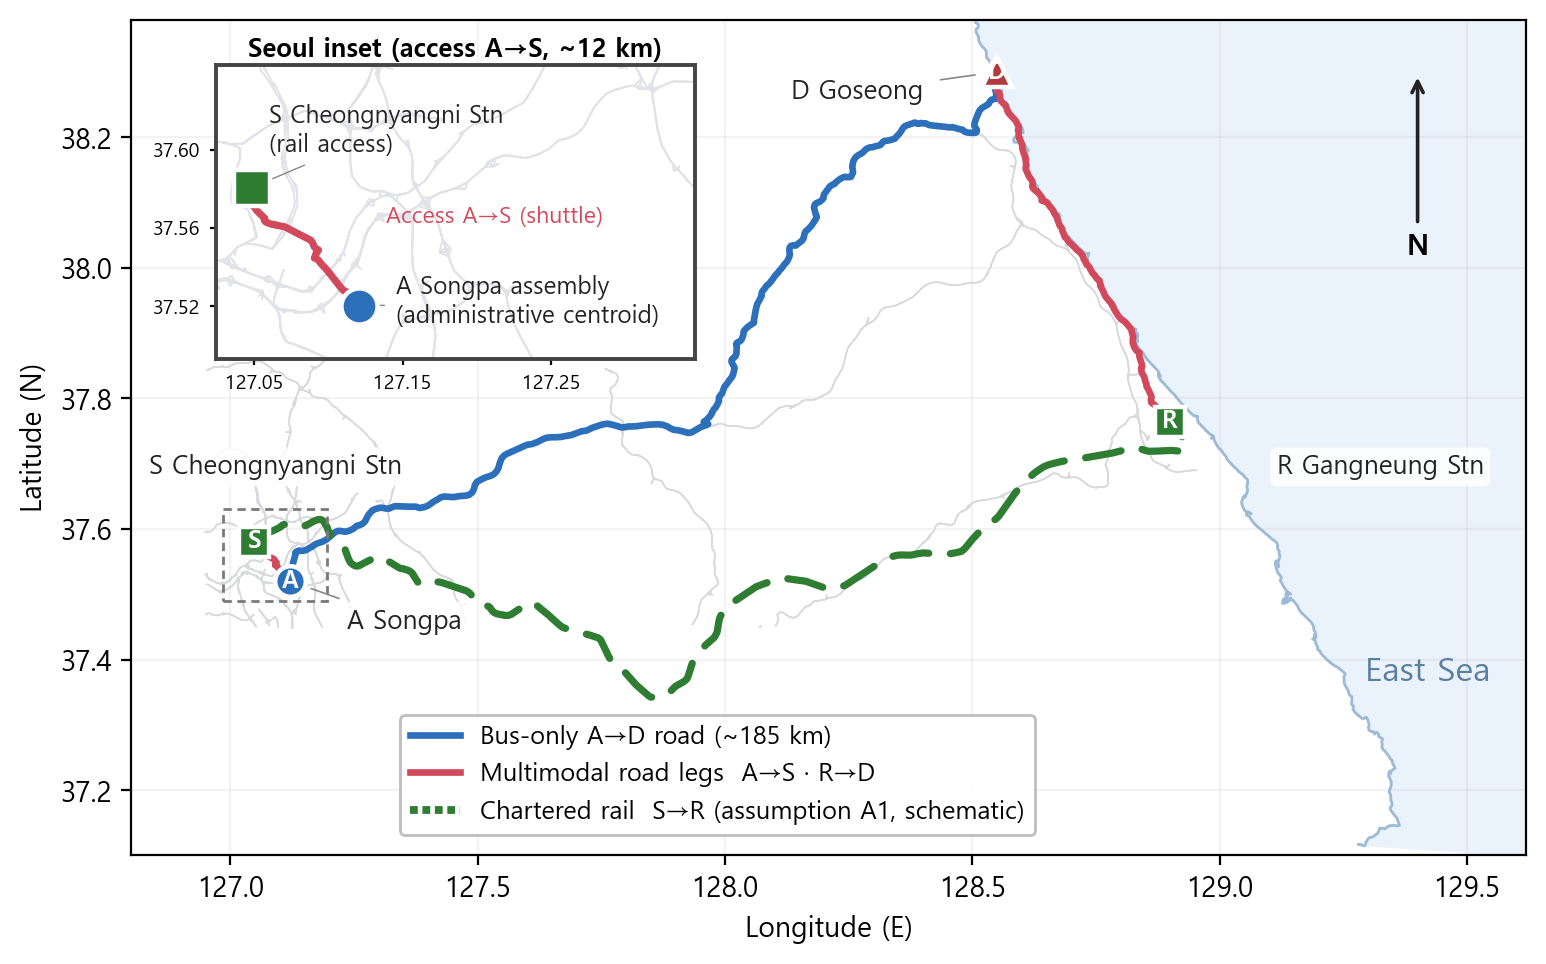
\includegraphics[width=\linewidth]{fig2.png}
\caption{Songpa--Goseong case corridor and exposure structure of the two transport configurations. Road centerlines derive from the Standard Node-Link cache; A, S, R, and D are public administrative centroids and public rail-station coordinates. Drawn links explain the comparison structure and are not a field movement plan.}
\label{fig:corridor}
\end{figure}

\section{Simulation Model}
\label{sec:model}

\subsection{Alternatives and outcome rule}
Both alternatives are discrete-event microsimulations over a 1{,}440 min horizon. Demand is 1{,}000 passengers at A with lognormal arrival fixture ($\mu=2.45$, $\sigma=0.75$; natural-log parameters in minutes, untruncated, added to assembly time $t=0$), boarding batch 45, origin share 1.0 at assembly time 0. The demand profile carries source class \texttt{sensitivity\_\allowbreak only}: the fixture scale is anchored to a published arrival-delay distribution shape and is not a calibrated origin--destination demand estimate. The outcome rule is lexicographic: maximize completion rate within the window; when completion rates match, minimize finite completion time. Incomplete runs are never converted into an arbitrary finite time penalty for the main ranking. This ordering follows the preference to separate completion failures from makespan comparisons rather than to mix them with a censoring constant. Completion rate is the fraction of the 1{,}000 passengers delivered at D by $t=1440$; makespan is the time of the last successful arrival when completion rate equals 1.0. When completion rates differ, makespan language is withheld even if one alternative records a finite mean time over its completed seeds. The lexicographic rule is applied uniformly to static policies, adaptive policies, and every campaign cell, so rankings never mix a completion failure with a finite-time comparison across policies.

The passenger flow is staged as assembly queue, road or rail leg, optional transfer, and arrival at D. Assembly wait, transfer wait, and rail wait are accumulated as separate passenger-minute KPIs so that a low makespan is not mistaken for a low waiting burden. Under the strict departure policy used in all reported paper campaigns, a vehicle departs on schedule with the passengers who have arrived by that instant; later arrivals wait for the next dispatch interval rather than delaying the manifest. Graceful dispatch variants exist in the engine for sensitivity work but are outside the reported campaign set.

\subsection{Resource frames}
Two resource frames are reported separately.

\emph{Configured bundle:} bus-only uses 23 direct road vehicles; static multimodal uses 23 feeder shuttles, 23 last-mile buses, and rail.

\emph{Equal total road fleet:} bus-only uses 23 direct road vehicles; static multimodal uses 12 feeder shuttles, 11 last-mile buses, and rail. This frame equalizes road-vehicle count only. Rail capacity, cost, and energy remain unmatched.

Fleet roles carry 45 seats per vehicle, 5 min dispatch interval, first departure at $t=0$, and 8 min turnaround after empty return. The fleet profile carries source class \texttt{public\_\allowbreak cited}: role sizes are bounded scenario assumptions drawn from public procurement and organization references, not an operating roster. Every road vehicle completes passenger travel, traverses the current reverse road network empty, and only then may be reused; if no reverse path exists, that vehicle cannot return. Empty-return mileage is therefore active rather than implicit. Formally, vehicle $v$ becomes available for a new trip only after the triple (unload, reverse-path traversal on the current disrupted graph $G'$, turnaround), where $G'$ is recomputed after each scenario overlay. Empty-return KPIs reported in Section~VI-G are \texttt{empty\_\allowbreak return\_\allowbreak trips}, \texttt{empty\_\allowbreak return\_\allowbreak minutes}, and \texttt{road\_\allowbreak vehicle\_\allowbreak cycles}; blocked return links can strand a vehicle even when the forward passenger path still exists.

Table~\ref{tab:frames} restates the two resource frames side by side with the road-vehicle totals that enter every comparison. The configured bundle is the natural reading of a planner who assigns a dedicated feeder fleet and a dedicated last-mile fleet on top of rail; the equal-road-fleet frame forces road-vehicle parity so that the time comparison is not a pure fleet-size artifact, while still granting multimodal an unmatched rail resource. Neither frame is an equal-cost frame; cost, energy, and crew accounting are outside scope.

\begin{table}[!t]
\caption{Resource frames (45 seats/vehicle; 5 min dispatch; 8 min turnaround after reverse empty return).}
\label{tab:frames}
\centering
\footnotesize
\begin{tabular}{@{}llrrr@{}}
\hline
Frame & Policy & Direct & Feeder+Last & Road total \\
\hline
Configured & bus-only & 23 & 0 & 23 \\
Configured & multimodal & 0 & 23+23 & 46 \\
Equal fleet & bus-only & 23 & 0 & 23 \\
Equal fleet & multimodal & 0 & 12+11 & 23 \\
\hline
\end{tabular}
\\
\footnotesize{Rail (600 pax/train, 30 min dispatch) is additional in both multimodal cells.}
\end{table}

\subsection{Rail service states}
Rail is a wartime chartered nonstop service from S to R with planning travel time 114 min, capacity 600 passengers per train, and 30 min dispatch interval---a charter dispatch assumption, not a public headway claim. Runtime anchors to public Gangneung Line KTX-Eum timetable material \cite{b18}. States are: \emph{available} (multiplier 1.0), \emph{degraded} (1.25, 1.5, or 2.0), and \emph{unavailable} (service out of the model, not an arbitrarily large travel time). The unavailable state removes the S$\rightarrow$R rail leg from the multimodal itinerary so that static multimodal without a fallback rule cannot deliver passengers past S when no road substitute is declared. Treating unavailability as an explicit state rather than as a very large travel time keeps completion-rate ranking separate from finite-makespan ranking. Adaptive policies may precheck-switch (detect rail outage and reassign the group to road before departure), split groups (600 by rail / 400 by road), or fall back to station transfer after 30/60/90 min of waiting. Degraded multipliers stretch rail travel time but do not remove the leg; only the unavailable state removes it.

\subsection{Road network dynamics and disruptions}
Edge free-flow times and capacities come from per-class overrides grounded in public capacity manuals and statutory speed limits \cite{b2,b3,b5,b16,b7}. For edge $e$ with free-flow time $t_0(e)$, capacity $C(e)$, and volume $V(e)$ in the rolling evaluation window, the link time is
\begin{equation}
t(e) = t_0(e)\bigl[1 + \alpha (V(e)/C(e))^{\beta}\bigr],
\label{eq:bpr}
\end{equation}
with BPR coefficients $\alpha=0.36$ and $\beta=4.0$ evaluated on a 60-min rolling volume window (the Korean-calibration-direction run value; the engine library default remains the FHWA $\alpha=0.15$). Under A2 the civilian background input of 100 veh/h is small relative to motorway through trunk capacities (3{,}600 down to 600 veh/h), so the multiplicative congestion term is near 1 by construction; a dedicated BPR no-op sweep confirms the inert behavior and is not repeated as an empirical traffic finding. Disruptions apply deterministic scenario overlays for paper campaigns: selected edges receive blocking (removed and rerouted), capacity reduction, or direct travel-time multipliers. Segment-targeted road damage uses a direct-slowdown lever (\texttt{travel\_\allowbreak time\_\allowbreak multiplier} on selected edges with capacity factor 1.0) so road damage is isolated from the wartime-inert BPR path. Targeting is by functional-segment shortest path: A$\rightarrow$S access damage bites the multimodal feeder leg; R$\rightarrow$D last-mile damage bites both alternatives; S$\rightarrow$R long-haul damage bites bus-only while multimodal substitutes rail under A1. The central long-haul target set contains 3{,}582 physical edges with matching checksums in top-10 and full scope. Blocked edges are removed and remaining routes are searched again with shortest-path recomputation on the residual graph \cite{b25}; a road leg fails only when no path remains. Transfer delay is modeled as a base 3.0 min plus 0.02 min per passenger, plus a waiting component that depends on the feeder arrival time relative to the next feasible connection; assembly wait, transfer wait, and rail wait are logged as separate passenger-minute KPIs. This residual-graph rerouting is why critical-link and fixed random-blockage cells complete rather than collapse.

\subsection{Discrete-event mechanics}
Passengers queue at assembly, board under strict dispatch policy (depart on time with arrived passengers only for all reported paper campaigns), travel road or rail legs with transfer delay, and unload at D. Makespan is the time of last successful arrival when completion rate is 1.0; completion rate is the fraction of demand delivered within 1{,}440 min. Resource KPIs include vehicle cycles, empty-return trips, empty-return minutes, road-vehicle operating minutes, bus trips, and rail trips. The event loop advances by departure, arrival, transfer, rail dispatch, and turnaround events; no continuous time-stepped link update is required beyond the rolling-window BPR evaluation, which is inert under A2. Each road vehicle's state machine is explicit: available at depot, assigned to a manifest, traversing a loaded leg, unloading, traversing a reverse empty leg on the current disrupted graph, then in turnaround. A vehicle stuck on a reverse empty leg with no residual path is marked unavailable for further reuse and is not silently teleported back to depot. This bookkeeping is what makes the empty-return KPIs in Table~\ref{tab:empties} interpretable: differences across frames reflect trip structure and leg lengths, not an implicit free return.

\section{Experimental Design}
\label{sec:design}

\subsection{Campaigns}
Fifteen campaign sets produced 29{,}940 runs on the top-10 graph, the full reference graph, and a second corridor (Table~\ref{tab:campaigns}). All campaigns use CRN seed blocks (arrival seeds 3101--3130 unless a campaign nests additional threat draws) and \texttt{force\_\allowbreak deterministic\allowbreak=True} within scenario. Fixed-scenario campaigns hold the threat set constant and vary arrival seeds. The random-threat campaign nests 30 arrival seeds inside each of 100 independently generated eight-edge threat sets. Campaign checkpoints make the full run resumable; bootstrap products reuse seed 20260721 throughout. The row inventory is reported so that a reader can reconstruct which campaign supports which table: baseline and paired stress cells come from paired reanalysis; the crossing and its fine bracket come from the two break-even campaigns; frame-by-rail-state claims come from the road--rail map; completion-stress claims come from demand--fleet and scale; policy rankings come from adaptive policies; screening and half-width claims come from Morris and replicate convergence; the zero-completion interdiction statement comes only from the path-interdiction campaign; allocation-conditional claims come from the allocation surface sweep; scope-stability claims for the boundary come from the full-graph break-even validation; assumption-conditional claims come from the break-even sensitivity set; and transferability claims come from the second-corridor case.

\begin{table}[!t]
\caption{Paper-revision campaigns (top-10 corridor graph).}
\label{tab:campaigns}
\centering
\footnotesize
\begin{tabular}{@{}lrr@{}}
\hline
Campaign & Design summary & Rows \\
\hline
Paired reanalysis & $21\times2\times2\times30$ & 2{,}520 \\
Graph scope & top-3/5/10/full & 1{,}330 \\
Break-even (coarse) & $16\times2\times2\times30$ & 1{,}920 \\
Break-even (fine) & $17\times2\times2\times30$ & 2{,}040 \\
Demand--fleet & $4\times4\times2\times2\times30$ & 1{,}920 \\
Scale sensitivity & $4\times1\times30\times2$ & 240 \\
Road--rail map & $6\times5\times2\times2\times30$ & 3{,}600 \\
Path interdiction & $2k\times10\times2\times2\times30$ & 2{,}400 \\
Random threat outer & $100\times30\times2$ & 6{,}000 \\
Adaptive policies & $3\times2\times7\times30$ & 1{,}260 \\
Morris & $(6+1)\times20\times5\times2$ & 1{,}400 \\
Allocation surface & 22 splits $\times 30$ + invariance $5\times30$ & 810 \\
Full-graph break-even & $7\times2\times2\times30$ + sanity/config & 1{,}080 \\
Break-even sensitivity & $3\times6\times30$ + $10\times30$ & 840 \\
Second corridor (Yangyang) & audit + frames + alloc + sweep & 2{,}590 \\
\hline
\textbf{Total} & & \textbf{29{,}940} \\
\hline
\end{tabular}
\end{table}

The road--rail map uses road multipliers 1.0, 1.2, 1.4, 1.6, 2.0, and 3.0 and rail conditions available 1.0, degraded 1.25/1.5/2.0, and unavailable. Adaptive policies use available 1.0, degraded 1.5, and unavailable. Break-even (coarse) spans 16 multipliers from 1.0 to 3.0; break-even (fine) refines the bracket with 17 multipliers including 1.70--1.78 at 0.01--0.02 spacing near the estimated crossing. Scale sensitivity tests demand 2{,}000, 6{,}000, 8{,}000, and 12{,}000 at the fixed-12/11 break-even road multiplier 1.742. Path interdiction uses budget-$k\in\{3,5\}$ edge removal on the A--D shortest path with blocked-edge recovery; those runs are retained in the campaign inventory, and their zero-completion outcome under the reduced corridor envelope is discussed only as a graph-scope-sensitive stress result, not as a break-even estimate. Campaign checkpoints write partial results to disk after each cell so an interrupted full run resumes without re-executing completed rows; \texttt{--no-resume} is reserved for deliberately isolated clean output roots.

\begin{figure}[!t]
\centering
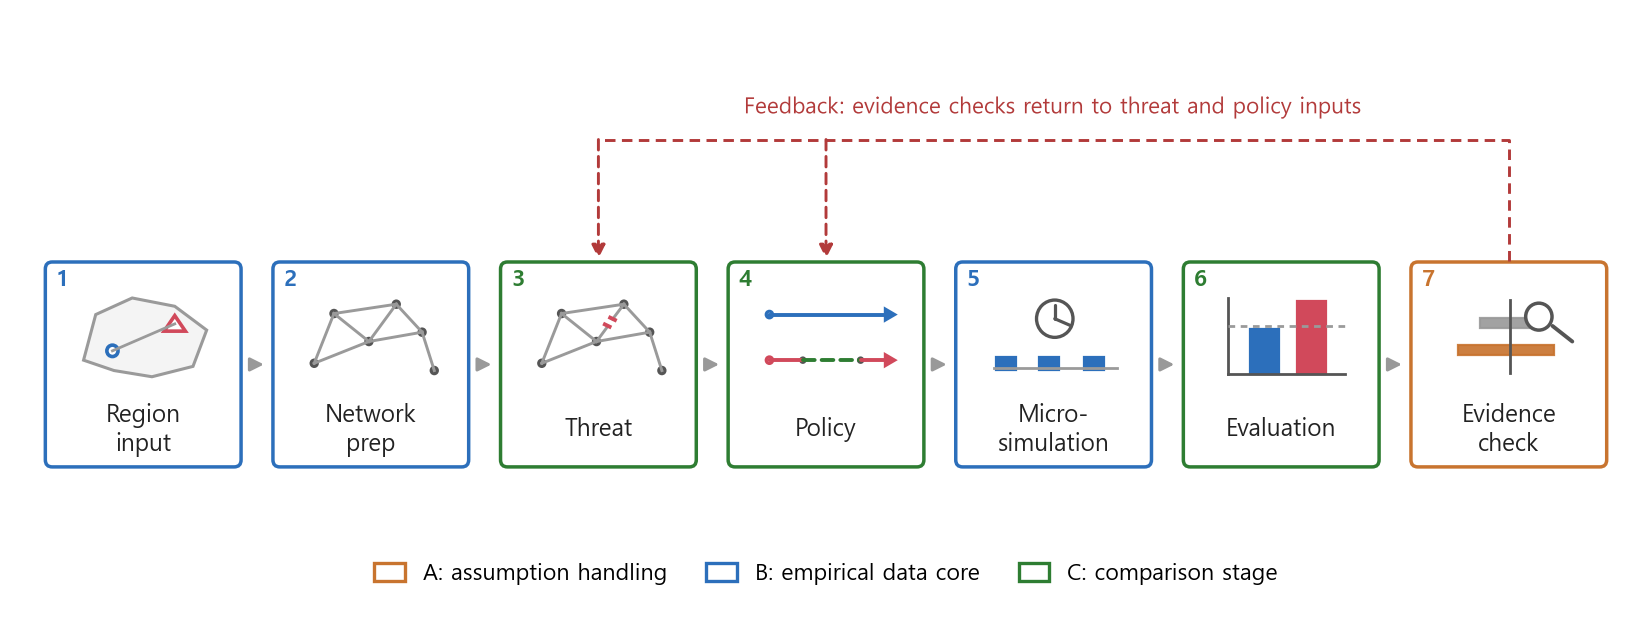
\includegraphics[width=\linewidth]{fig1.png}
\caption{Research procedure and feedback structure. Public regional inputs and road-network preparation lead to threat and policy definition, microsimulation, alternative evaluation, and evidence checks with sensitivity analysis; closing checks feed back into threat and policy inputs.}
\label{fig:procedure}
\end{figure}

\subsection{Inference rules}
For each configuration and seed $s$ with equal completion rates and finite makespans,
\begin{equation}
\Delta_s = MS_{\mathrm{bus},s} - MS_{\mathrm{multi},s}.
\label{eq:delta}
\end{equation}
Negative $\Delta$ favors bus-only on completion time; positive $\Delta$ favors static multimodal. We report paired-$t$ 95\% intervals and 10{,}000-replicate percentile bootstrap intervals. Break-even uses linear interpolation of mean $\Delta$ across road multipliers bracketing a sign change, with a joint-seed bootstrap (10{,}000 replicates over complete seeds) for the crossing. The coarse break-even campaign uses 16 multipliers from 1.0 to 3.0; the fine campaign uses 17 multipliers including 0.01--0.02 spacing between 1.72 and 1.78 so that the sign change is bracketed by adjacent grid points rather than only by the 1.6/1.8 endpoints. The random-threat campaign reuses the same 30 arrival seeds across all 100 threat draws (crossed factors), so the primary uncertainty product is a crossed two-way bootstrap: each replicate resamples 100 threat draws with replacement and resamples the 30 arrival-seed IDs globally once, averaging the resampled Cartesian submatrix with policy pairing preserved cell-wise (3{,}000 finite pairs). A nested two-level variant (independent seed resampling within each resampled draw) is retained for comparison only, because it destroys the cross-threat seed dependence. Replicate-count tables at 5/10/20/30 prevent a blanket claim that 30 runs are universally adequate. Completion frequencies of 1.0 describe generated simulation draws, not real-event probabilities. Sensitivity statements follow the separation between screening importance and calibrated sensitivity advocated in the simulation-experiment literature \cite{b22,b23}. All bootstrap products use seed 20260721 and are stored with the analysis CSVs referenced in Section~X. A completion ranking is reported as resolved only when both the paired-$t$ and the percentile-bootstrap interval for the seed-paired completion difference $d_s=C_{\mathrm{bus},s}-C_{\mathrm{multi},s}$ exclude zero in the same direction (or both collapse to exactly zero, a resolved tie); otherwise the cell is unresolved. Capacity-saturated cells whose per-seed completion is identical across all seeds yield point intervals by construction, and are reported as deterministic capacity effects rather than sampling noise.

\subsection{Graph-scope audit}
For seven configured-bundle scenarios $\times$ five common seeds, connectivity agreement uses 70 outcomes and policy-ranking agreement uses 35 bus-versus-static comparisons against the full reference graph. Functional-segment normal times are compared for A$\rightarrow$D, A$\rightarrow$S, R$\rightarrow$D, and S$\rightarrow$R. The central long-haul target contains 3{,}582 physical edges with matching checksums in top-10 and full scope; extreme multipliers are checked for top-10/full A$\rightarrow$D travel-time ratio via the corridor-target scope metrics. Table~\ref{tab:legtimes} reports functional-segment normal travel times by scope: A$\rightarrow$D, A$\rightarrow$S, and R$\rightarrow$D are identical across top-3, top-5, top-10, and full (exact shortest simple paths are shared), while only S$\rightarrow$R separates the scopes. The audit is an agreement study against a fixed reference, not a claim that the full graph is ground truth for wartime conditions.

\begin{table}[!t]
\caption{Functional-segment normal travel times (min) by graph scope (undamaged free-flow shortest paths).}
\label{tab:legtimes}
\centering
\footnotesize
\begin{tabular}{@{}lrrrr@{}}
\hline
Scope & A$\rightarrow$D & A$\rightarrow$S & R$\rightarrow$D & S$\rightarrow$R \\
\hline
top-3 & 129.2 & 15.1 & 61.4 & 170.9 \\
top-5 & 129.2 & 15.1 & 61.4 & 146.0 \\
top-10 & 129.2 & 15.1 & 61.4 & 142.4 \\
full & 129.2 & 15.1 & 61.4 & 140.3 \\
\hline
\end{tabular}
\end{table}

\section{Results}
\label{sec:results}

\subsection{Baseline by resource frame}
Table~\ref{tab:baseline} reports the no-disruption (and access-segment) baseline on the top-10 graph. Under the configured bundle the point estimate favors multimodal by about 10 min, but both the $t$ and bootstrap intervals include zero. Under the equal total road fleet with the fixed 12-feeder/11-last-mile split, bus-only is about 102 min faster with intervals far from zero. Resource definition therefore changes the baseline interpretation before any disruption is applied. The sign flip is not a statistical artifact of a single seed block: the same CRN pairs yield opposite frame conclusions under the two counting rules. Mechanically, the configured-bundle multimodal alternative receives 23 feeder and 23 last-mile road vehicles in addition to rail, so its road capacity roughly doubles while the bus-only side stays at 23 direct buses; equalizing total road vehicles at 23 removes that road-capacity subsidy but leaves the rail leg untouched. The unresolved configured-bundle interval is therefore not evidence of equality---it is evidence that thirty paired seeds cannot separate a +10 min mean at the observed within-pair variance.

The 12/11 equal-fleet split, however, is one arbitrary allocation, and it is far from the achievable frontier. Table~\ref{tab:alloc} sweeps all 23 feasible feeder/last-mile divisions of the 23-vehicle multimodal budget at the no-disruption baseline (30 seeds each, top-10). Mean multimodal makespan is U-shaped in the feeder share: starving either leg inflates completion time (1{,}094 min at 1/22, 1{,}152 min at 20/3), while splits 4--10 all complete with means between 394.6 and 412.1 min. The best split is 6 feeder + 17 last-mile at 394.6 min, about 80 min faster than the fixed 12/11 split at 475.8 min. Against the best split, the bus advantage shrinks to $-20.5$ min with paired intervals $[-44.2,\ 3.2]$ ($t$) and $[-44.8,\ 0.7]$ (bootstrap)---unresolved. The equal-road-fleet baseline is therefore itself allocation-conditional: bus-only is resolved faster than badly split multimodal fleets and statistically tied with well-split ones. Reporting a single 12/11 number as ``the'' equal-fleet comparison suppresses exactly the kind of resource-definition sensitivity this article argues must stay visible; the full 22-split surface ships with the analysis files.

Table~\ref{tab:empties} reports empty-return and vehicle-cycle KPIs at the no-disruption baseline. Under either frame, bus-only records about 24.3 empty-return trips and 3{,}135 empty-return minutes on average, while static multimodal records about 47.9 empty-return trips but only about 1{,}819 empty-return minutes on the feeder/last-mile legs (shorter per-trip returns) plus about 365 passenger bus-minutes and about 5.7 rail trips. Road-vehicle operating minutes are about 6{,}269 for bus-only versus about 3{,}638 for multimodal: the multimodal alternative spends fewer road operating minutes because the long haul is carried by rail, even though it cycles more short road trips. These KPIs make reverse empty return observable rather than implicit; without them the fixed-12/11 102 min gap would look like a pure passenger-leg effect rather than a consequence of matching road-vehicle counts while leaving rail unmatched.

\begin{table}[!t]
\caption{Baseline mean completion time (min) and paired difference $\Delta$ = bus $-$ multimodal (30 CRN pairs, top-10, reverse empty return, strict dispatch).}
\label{tab:baseline}
\centering
\footnotesize
\begin{tabular}{@{}lrrrr@{}}
\hline
Frame & Bus & Multi. & Mean $\Delta$ & $t$ 95\% CI \\
\hline
Configured bundle & 374.1 & 363.8 & $+10.3$ & $[-12.6,\ 33.2]$ \\
Equal road fleet (12/11 split) & 374.1 & 475.8 & $-101.7$ & $[-125.0,\ -78.4]$ \\
\hline
\end{tabular}
\end{table}

\begin{table}[!t]
\caption{Equal-road-fleet multimodal makespan by feeder/last-mile split (means over 30 seeds; top-10, no disruption, available rail) with paired bus-minus-multimodal difference and $t$ 95\% interval. Splits 5--10 form the robust band; 6/17 is fastest.}
\label{tab:alloc}
\centering
\footnotesize
\begin{tabular}{@{}rrrrr@{}}
\hline
Feeder/last-mile & Multi.\ MS & Comp. & Mean $\Delta$ & $t$ 95\% CI \\
\hline
1/22 & 1094.4 & 1.00 & $-720.4$ & $[-739.8,\ -700.9]$ \\
4/19 & 437.1 & 1.00 & $-63.0$ & $[-86.1,\ -40.0]$ \\
5/18 & 401.6 & 1.00 & $-27.5$ & $[-51.4,\ -3.6]$ \\
6/17 & 394.6 & 1.00 & $-20.5$ & $[-44.2,\ 3.2]$ \\
8/15 & 402.7 & 1.00 & $-28.7$ & $[-52.5,\ -4.9]$ \\
10/13 & 412.1 & 1.00 & $-38.0$ & $[-61.7,\ -14.4]$ \\
12/11 & 475.8 & 1.00 & $-101.7$ & $[-125.0,\ -78.4]$ \\
15/8 & 528.6 & 1.00 & $-154.5$ & $[-178.2,\ -130.9]$ \\
20/3 & 1151.7 & 1.00 & $-777.6$ & $[-800.2,\ -755.1]$ \\
22/1 & 1384.2 & 0.45 & $-1010.1$ & $[-1035.3,\ -984.9]$ \\
\hline
\end{tabular}
\end{table}

\begin{table}[!t]
\caption{No-disruption empty-return and resource KPIs (means over 30 seeds; top-10).}
\label{tab:empties}
\centering
\footnotesize
\begin{tabular}{@{}llrrr@{}}
\hline
Frame / policy & Empty trips & Empty min & Cycles & Road ops \\
\hline
Conf.\ bus-only & 24.3 & 3134.7 & 24.3 & 6269.5 \\
Conf.\ multi. & 47.9 & 1819.2 & 47.9 & 3638.4 \\
Equal bus-only & 24.3 & 3134.7 & 24.3 & 6269.5 \\
Equal multi. & 47.9 & 1819.2 & 47.9 & 3638.4 \\
\hline
\end{tabular}
\\
\footnotesize{Conf.\ = configured bundle; multi.\ = static multimodal (makespans in Table~\ref{tab:baseline}); road ops in minutes.}
\end{table}

\begin{figure}[!t]
\centering
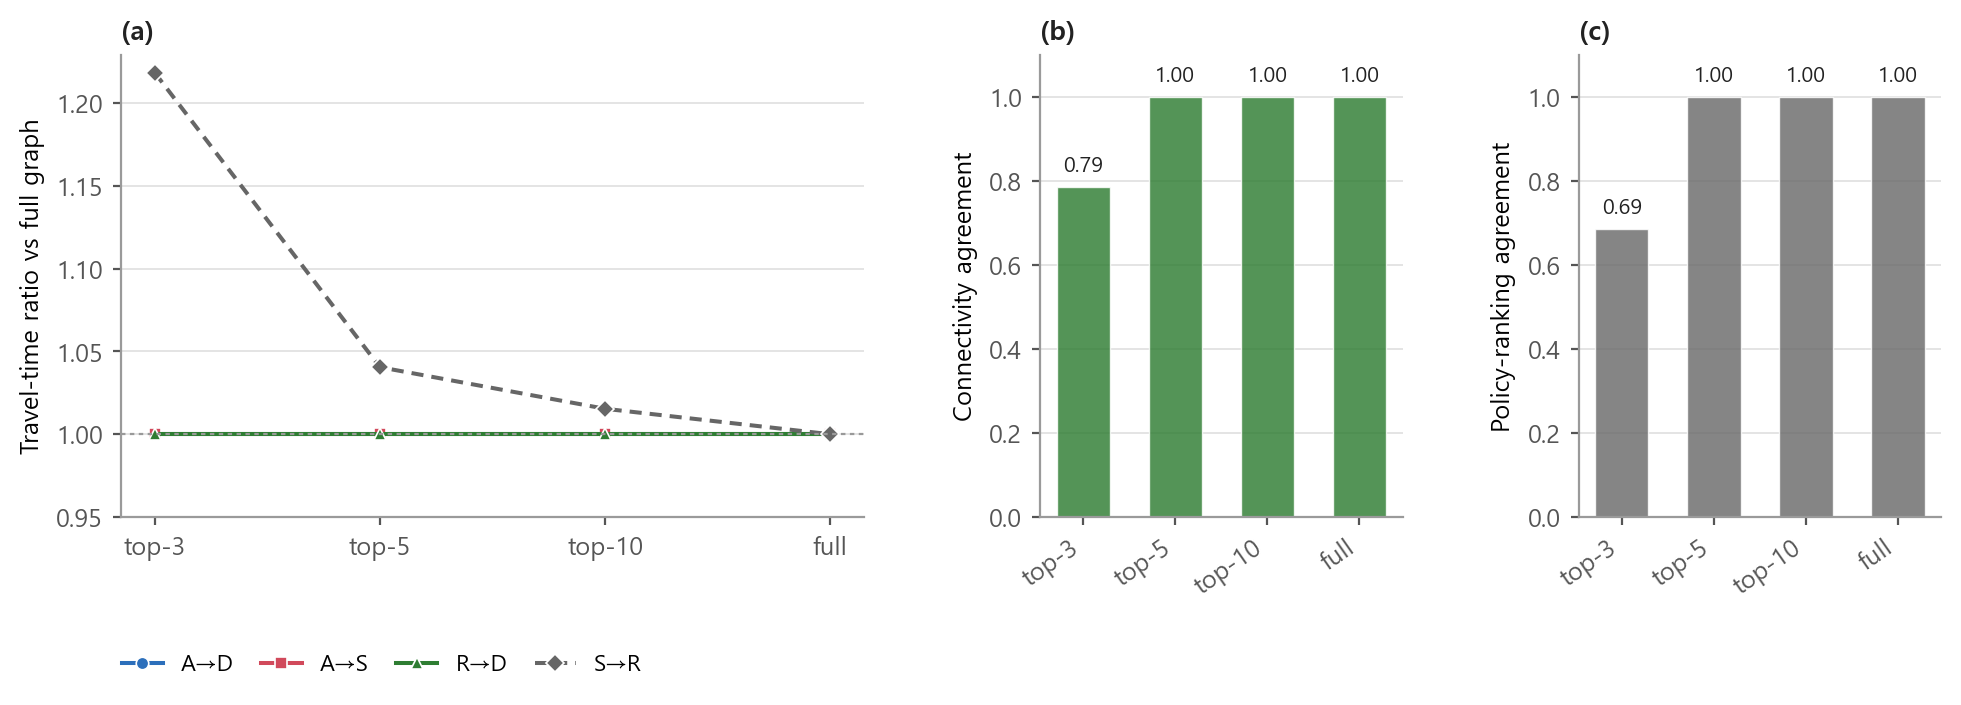
\includegraphics[width=\linewidth]{fig3.png}
\caption{Reduced-graph scope sensitivity. (a) Functional-segment travel-time ratios of top-3, top-5, and top-10 envelopes versus the full reference graph; (b) connectivity agreement (70 outcomes) and (c) bus--static policy-ranking agreement (35 comparisons) under seven configured-bundle scenarios and five common seeds. Top-5 and top-10 equal 1.00 on both agreements; top-3 is 0.786 and 0.686. S$\rightarrow$R normal-time ratios are 1.218 (top-3) and 1.015 (top-10). Results hold only for the tested conditions.}
\label{fig:scope}
\end{figure}

\subsection{Graph-scope audit}
Table~\ref{tab:scope} and Fig.~\ref{fig:scope} show that top-5 and top-10 preserve full-scope connectivity and bus-versus-static ranking in the tested conditions, while top-3 does not. Top-3 S$\rightarrow$R normal time is 1.218$\times$ full and top-10 is 1.015$\times$. At a 3.0 long-haul road multiplier, the top-10/full A$\rightarrow$D travel-time ratio reaches 1.157, so the extreme point is treated as a graph-scope boundary. The connectivity disagreement for top-3 is concentrated in stress cells where the missing diversified long-haul alternatives force a residual path that does not exist in the full graph's preferred corridor; ranking disagreement follows from the same residual structure because one alternative fails connectivity while the other completes. This audit does not directly re-prove the equal-road-fleet conclusion on the full graph; it bounds how far the reduced envelope may be trusted for the tested stress set. Practical reading: envelopes at least as large as top-5 are required before connectivity-based claims are reported on this corridor construction; top-3 is insufficient for ranking claims even though its normal-time error on A$\rightarrow$D, A$\rightarrow$S, and R$\rightarrow$D looks small. The 1{,}330 graph-scope rows are seven scenarios $\times$ two policies $\times$ (three reduced scopes $\times$ 30 arrival seeds $+$ full scope $\times$ 5 common seeds); the connectivity and ranking agreement products use the five common seeds.

\begin{table}[!t]
\caption{Graph-scope agreement with the full reference graph (configured bundle, seven scenarios, five seeds).}
\label{tab:scope}
\centering
\footnotesize
\begin{tabular}{@{}lrrrr@{}}
\hline
Scope & Nodes & Edges & Connectivity & Ranking \\
\hline
top-3 & 752 & 1{,}512 & 0.786 & 0.686 \\
top-5 & 2{,}733 & 5{,}532 & 1.000 & 1.000 \\
top-10 & 9{,}089 & 18{,}602 & 1.000 & 1.000 \\
full & 360{,}556 & 971{,}680 & ref. & ref. \\
\hline
\end{tabular}
\end{table}

\subsection{Segment-targeted stress under the equal road fleet}
Table~\ref{tab:stress} summarizes key equal-road-fleet stress cells. Critical-link and fixed random-blockage cases still complete for both alternatives after rerouting; they do not support a network-collapse claim on this graph. Long-haul slowdown moves $\Delta$ from clearly negative (bus faster) at mild/moderate damage toward positive at 3.0$\times$, where multimodal becomes faster because rail bypasses the shared trunk. Access-severe and last-mile-severe cells remain negative (bus still faster) under the equal-road-fleet frame because those legs do not by themselves overcome the unmatched-but-fixed multimodal feeder/last-mile split under available rail. Rail unavailability yields completion 1.00 versus 0.00, so makespan comparison is withheld (completion mismatch).

Table~\ref{tab:stressconf} reports the same stress cells under the configured bundle for contrast. Here almost every finite cell favors multimodal on makespan (positive $\Delta$), including mild access and last-mile damage, because the doubled road bundle more than absorbs those segment costs while rail still carries the long haul. Long-haul severe damage is the largest configured-bundle gap ($\Delta \approx +286$ min) and is significant under both $t$ and bootstrap intervals. The paired reading of Tables~\ref{tab:stress} and~\ref{tab:stressconf} is the central reporting-protocol result: the same scenario rows reverse or preserve the modal story depending only on how road resources are counted. Access-severe and last-mile-severe cells are especially diagnostic under the equal-road-fleet frame: those segments bite both alternatives, yet the multimodal feeder/last-mile split of 12+11 still cannot recover the unmatched rail benefit enough to flip $\Delta$ positive, whereas under the configured bundle the same segment damage leaves a comfortable multimodal margin. Segment targeting therefore does not by itself determine the winner; the frame in which the segment damage is evaluated does.

\begin{table}[!t]
\caption{Equal-road-fleet stress results at the fixed 12/11 split (top-10; completion rates and mean $\Delta$ with bootstrap 95\% interval where both complete).}
\label{tab:stress}
\centering
\footnotesize
\begin{tabular}{@{}lccrr@{}}
\hline
Scenario & Comp.\ bus/multi. & Mean $\Delta$ & Bootstrap CI \\
\hline
No disruption & 1.00/1.00 & $-101.7$ & $[-126.0,\ -81.0]$ \\
Access severe & 1.00/1.00 & $-106.5$ & $[-128.8,\ -87.0]$ \\
Last-mile severe & 1.00/1.00 & $-113.8$ & $[-139.4,\ -92.1]$ \\
Long-haul 1.2$\times$ & 1.00/1.00 & $-74.3$ & $[-100.9,\ -51.6]$ \\
Long-haul 1.5$\times$ & 1.00/1.00 & $-33.2$ & $[-63.3,\ -7.3]$ \\
Long-haul 3.0$\times$ & 1.00/1.00 & $+173.7$ & $[125.5,\ 215.1]$ \\
Critical-link block & 1.00/1.00 & $-103.6$ & $[-128.1,\ -82.7]$ \\
Rail unavailable & 1.00/0.00 & --- & --- \\
\hline
\end{tabular}
\end{table}

\begin{table}[!t]
\caption{Configured-bundle stress results (top-10; mean $\Delta$ with $t$ 95\% interval where both complete).}
\label{tab:stressconf}
\centering
\footnotesize
\begin{tabular}{@{}lccr@{}}
\hline
Scenario & Comp.\ bus/multi. & Mean $\Delta$ & $t$ CI \\
\hline
No disruption & 1.00/1.00 & $+10.3$ & $[-12.6,\ 33.2]$ \\
Access mild & 1.00/1.00 & $+10.4$ & $[-12.9,\ 33.7]$ \\
Access severe & 1.00/1.00 & $+16.1$ & $[-7.6,\ 39.9]$ \\
Access extreme & 1.00/1.00 & $+17.2$ & $[-7.7,\ 42.2]$ \\
Last-mile mild & 1.00/1.00 & $+10.7$ & $[-12.5,\ 33.9]$ \\
Last-mile severe & 1.00/1.00 & $+13.6$ & $[-10.2,\ 37.5]$ \\
Last-mile extreme & 1.00/1.00 & $+20.3$ & $[-5.1,\ 45.7]$ \\
Long-haul mild & 1.00/1.00 & $+37.7$ & $[12.5,\ 62.9]$ \\
Long-haul moderate & 1.00/1.00 & $+78.8$ & $[50.0,\ 107.6]$ \\
Long-haul severe & 1.00/1.00 & $+285.7$ & $[240.3,\ 331.1]$ \\
Critical-link block & 1.00/1.00 & $+11.5$ & $[-11.6,\ 34.6]$ \\
Rail unavailable & 1.00/0.00 & --- & --- \\
\hline
\end{tabular}
\end{table}

\begin{figure}[!t]
\centering
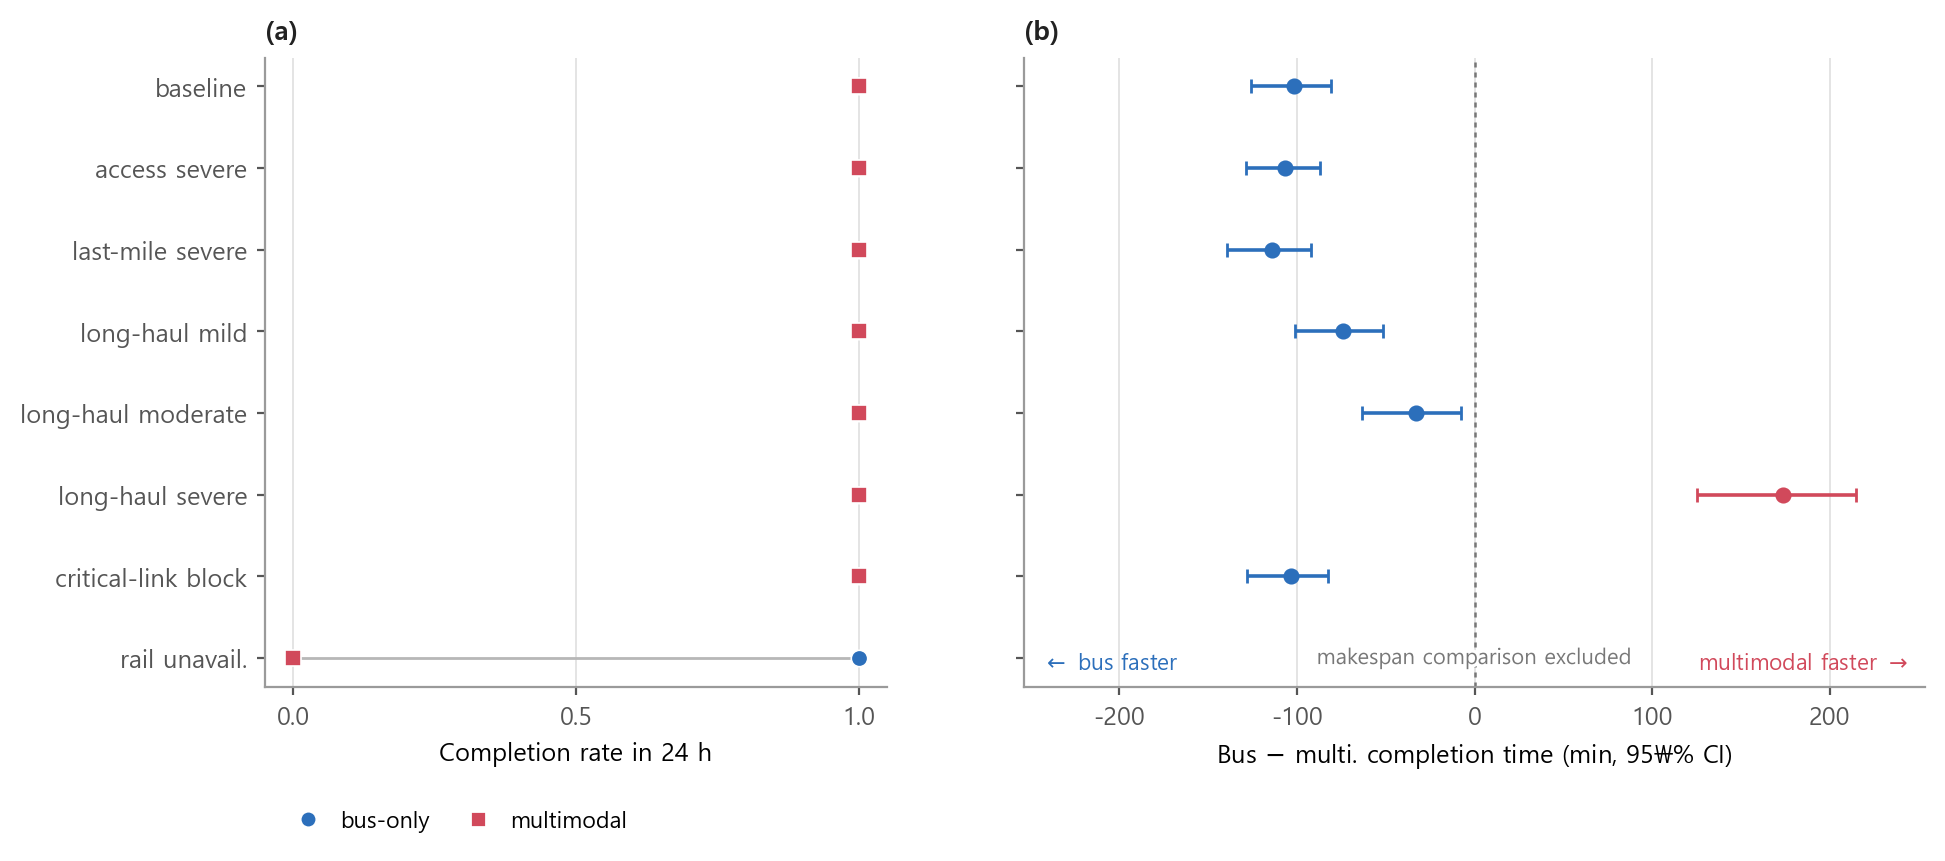
\includegraphics[width=\linewidth]{fig4.png}
\caption{Equal-road-fleet paired stress comparison at the fixed 12/11 split (top-10, reverse empty return, 30 CRN seeds; road-vehicle totals matched, rail cost not matched). (a) Completion rate within 24 h; (b) mean completion-time difference $\Delta$ = bus-only $-$ static multimodal with percentile-bootstrap 95\% intervals. Negative values favor bus-only; positive values favor multimodal. Only the extreme long-haul damage cell flips the time ordering; rail-unavailable cells are ranked on completion rate only. Allocation-conditional baselines are reported in Table~\ref{tab:alloc}.}
\label{fig:stress}
\end{figure}

\subsection{Break-even boundary}
In the equal-road-fleet frame with normally available rail, mean $\Delta$ for the fixed 12/11 split changes from $-19.49$ min at 1.6$\times$ long-haul road slowdown to $+7.91$ min at 1.8$\times$. Linear interpolation gives a crossing of 1.742. The joint-seed bootstrap 95\% interval is $[1.550,\ 2.003]$ (10{,}000 replicates; 30 complete seeds). Table~\ref{tab:be} reports the coarse and fine grids side by side. The fine grid (17 multipliers) places the sign change between 1.74 ($\Delta=-0.31$) and 1.75 ($\Delta=+1.06$), with interpolated crossing 1.742---consistent with the coarse estimate and now bracketed by adjacent grid points rather than only by the 1.6/1.8 endpoints. The configured-bundle curve has no zero crossing on 1.0--3.0 because mean $\Delta$ is already positive at 1.0 and increases monotonically to about $+286$ min at 3.0. Mechanically, a crossing exists because only the bus-only itinerary uses the S$\rightarrow$R road trunk; slowing that trunk raises bus makespan while the rail-bypass alternative is first-order insensitive to road multipliers on S$\rightarrow$R under A1 (its mean is 475.76 min at every tested multiplier for the 12/11 split).

The 1.742 estimate, however, belongs to one fixed allocation, not to the equal-road-fleet frame. Because the multimodal side is multiplier-invariant, each feasible split has its own crossing where the shared bus-only curve meets that split's flat multimodal mean. Table~\ref{tab:band} reports crossings with joint-seed intervals for the robust band and the legacy split: splits 5--10 cross between 1.150 and 1.277, while 12/11 crosses at 1.742. The headline boundary is therefore an allocation-dependent band, not a point: under normally available rail and demand 1{,}000, planners using a well-split multimodal fleet face a crossing near 1.15--1.28, and only the 12/11 policy pushes it to 1.74. Within the joint-seed intervals, equal-road-fleet planners who believe long-haul slowdown stays below about 1.0$\times$ retain a bus advantage on mean completion time; those who believe it exceeds about 1.5$\times$ see a multimodal advantage against robust splits; the middle band is unresolved at this replication count.

\begin{table}[!t]
\caption{Fixed-12/11-split mean $\Delta$ (bus $-$ multi., min) on coarse and fine break-even grids (top-10, available rail, 30 seeds). Crossing 1.742; joint-seed bootstrap 95\% interval $[1.550,\ 2.003]$.}
\label{tab:be}
\centering
\footnotesize
\begin{tabular}{@{}rr@{\qquad}rr@{}}
\hline
Road mult. & Mean $\Delta$ & Road mult. & Mean $\Delta$ \\
\hline
1.00 & $-101.71$ & 1.70 & $-5.79$ \\
1.20 & $-74.30$ & 1.72 & $-3.05$ \\
1.40 & $-46.90$ & 1.74 & $-0.31$ \\
1.50 & $-33.19$ & 1.75 & $+1.06$ \\
1.60 & $-19.49$ & 1.76 & $+2.43$ \\
1.80 & $+7.91$ & 1.78 & $+5.17$ \\
2.00 & $+35.45$ & 2.00 & $+35.45$ \\
3.00 & $+173.69$ & 3.00 & $+173.69$ \\
\hline
\end{tabular}
\end{table}

\begin{table}[!t]
\caption{Allocation-dependent break-even crossings (top-10, available rail, 30 seeds): interpolated crossing with joint-seed bootstrap 95\% interval per feeder split.}
\label{tab:band}
\centering
\footnotesize
\begin{tabular}{@{}rrrr@{}}
\hline
Feeder/last-mile & Multi.\ mean & Crossing & Joint 95\% CI \\
\hline
5/18 & 401.6 & 1.201 & $[1.048,\ 1.416]$ \\
6/17 & 394.6 & 1.150 & $[1.018,\ 1.362]$ \\
10/13 & 412.1 & 1.277 & $[1.115,\ 1.499]$ \\
12/11 & 475.8 & 1.742 & $[1.550,\ 2.003]$ \\
\hline
\end{tabular}
\end{table}

\begin{figure}[!t]
\centering
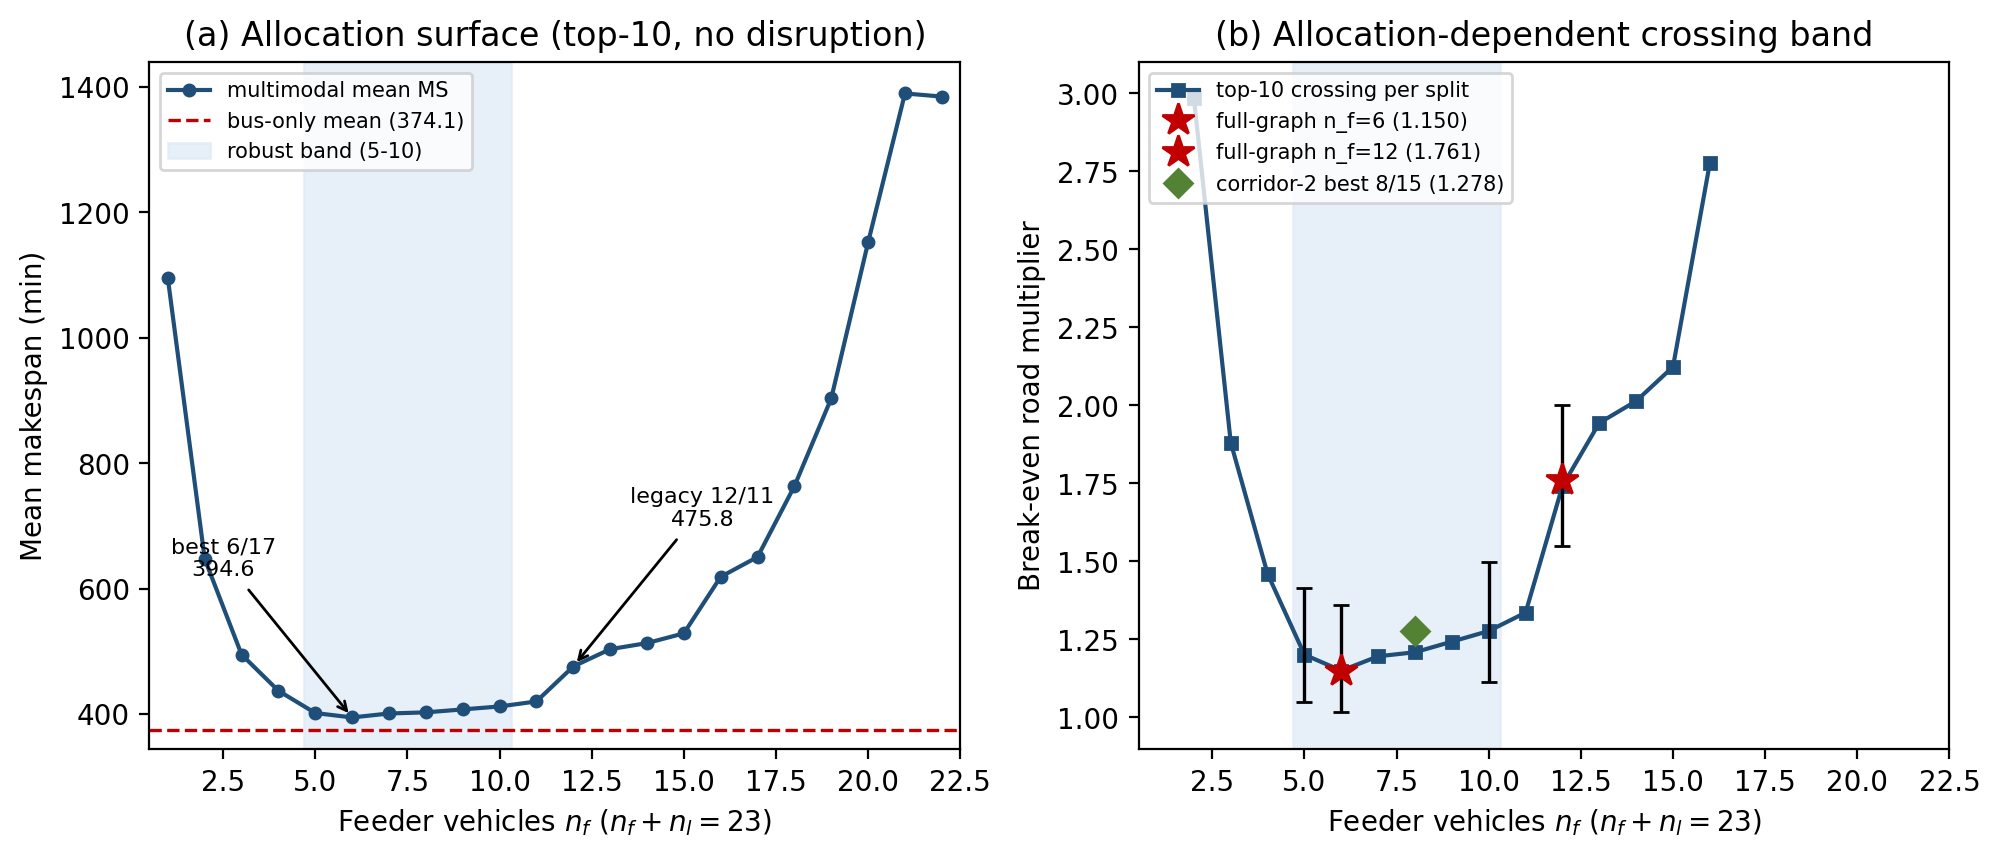
\includegraphics[width=\linewidth]{fig7.png}
\caption{Allocation-conditional boundary (top-10, matched road fleet, available rail, 30 seeds). (a) Mean multimodal makespan across all 23 feasible feeder/last-mile splits at no disruption; dashed line is the bus-only mean (374.1 min) and shading marks the robust band (splits 5--10). (b) Break-even crossing per split with joint-seed 95\% intervals at splits 5, 6, 10, and 12; red stars are full-graph validation points and the green diamond is the second-corridor crossing at its own best split. The crossing sweeps from about 1.15 to 2.78 across feasible splits.}
\label{fig:band}
\end{figure}

\begin{figure}[!t]
\centering
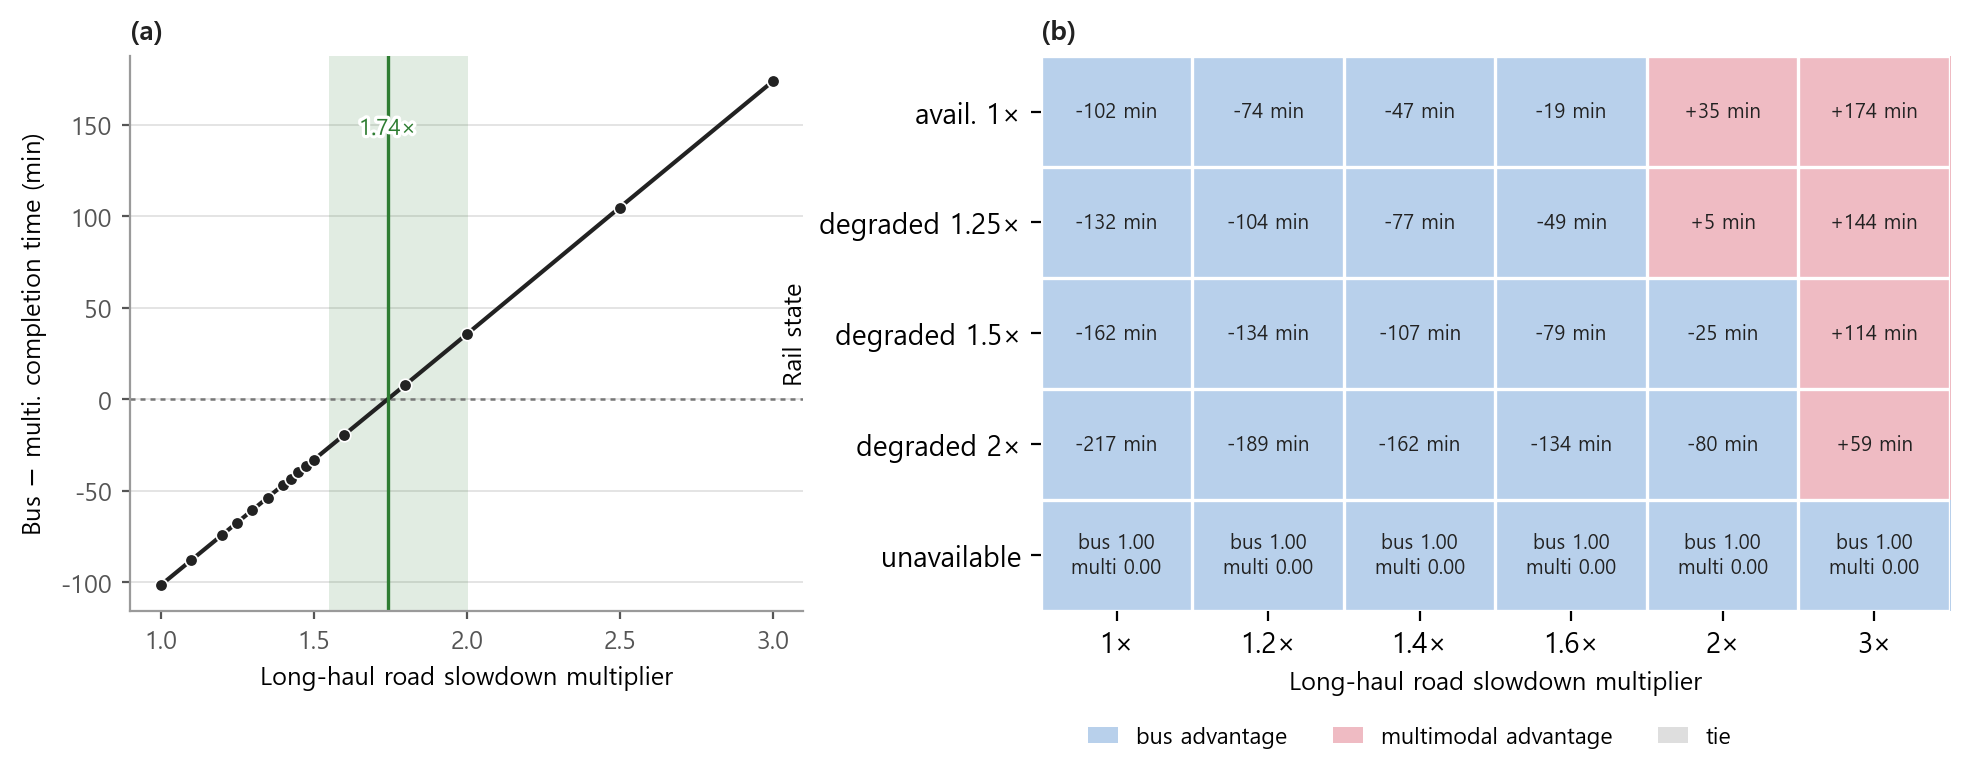
\includegraphics[width=\linewidth]{fig5.png}
\caption{Fixed-12/11-split road--rail decision boundary (top-10, reverse empty return, 30 CRN seeds). (a) Mean completion-time difference versus long-haul road multiplier with normally available rail; interpolated crossing 1.742 with joint-seed bootstrap 95\% interval 1.550--2.003. (b) Technical winner across road slowdown and rail-state combinations; cells with both alternatives complete show time difference, rail-unavailable cells show completion rates. The crossing is conditional on the stated demand, resource frame, rail state, and the fixed 12/11 fleet split; the allocation-dependent band is reported in Table~\ref{tab:band}.}
\label{fig:boundary}
\end{figure}

\subsection{Full-graph validation of the boundary}
The headline crossings are top-10 results, so a focused break-even grid was re-run on the full reference graph (360{,}556 nodes; 971{,}680 edges) with the same CRN seeds: multipliers 1.50--2.00 for the matched frame at the best (6/17) and legacy (12/11) splits, plus configured-bundle sanity cells at 1.0 and 3.0 (1{,}080 runs). The long-haul band re-derived on the full graph contains the same 3{,}582 edges with matching checksums. Multimodal means are identical across scopes to two decimals (475.76 min for 12/11 and 394.57 min for 6/17 at every multiplier on both graphs), confirming the structural multiplier-invariance on the full graph as well. Table~\ref{tab:fullbe} compares paired mean $\Delta$ curves: the 12/11 full-graph crossing is 1.761 with joint interval $[1.555,\ 1.989]$, a displacement of only $+0.019$ against the top-10 1.742 $[1.550,\ 2.003]$; the 6/17 full-graph crossing is 1.150 with joint interval $[1.106,\ 1.389]$, matching the top-10 point estimate exactly. Configured-bundle sanity cells agree at 1.0 ($+10.3$ min on both graphs) and differ only at the extreme 3.0 ($+216.3$ full versus $+285.7$ top-10), where the full graph's richer residual structure reroutes better. The reduced-envelope boundary therefore survives full-graph validation inside its reported uncertainty, and the allocation-band ordering (robust splits near 1.15--1.28, fixed 12/11 near 1.74--1.76) is scope-stable.

\begin{table}[!t]
\caption{Paired mean $\Delta$ (bus $-$ multi., min) on top-10 versus full graph by feeder split (available rail, 30 seeds). The 6/17 full-graph crossing uses additional bus-only cells at 1.1--1.4.}
\label{tab:fullbe}
\centering
\footnotesize
\begin{tabular}{@{}r@{\quad}rr@{\quad}rr@{}}
\hline
Road mult. & \multicolumn{2}{c}{6/17 split} & \multicolumn{2}{c}{12/11 split} \\
 & top-10 & full & top-10 & full \\
\hline
1.10 & $-6.8$ & $-6.8$ & $-88.0$ & $-88.0$ \\
1.20 & $+6.9$ & $+6.9$ & $-74.3$ & $-74.3$ \\
1.50 & $+48.0$ & $+46.7$ & $-33.2$ & $-34.5$ \\
1.60 & $+61.7$ & $+59.9$ & $-19.5$ & $-21.3$ \\
1.74 & $+80.9$ & $+78.4$ & $-0.3$ & $-2.8$ \\
1.75 & $+82.2$ & $+79.7$ & $+1.1$ & $-1.5$ \\
1.80 & $+89.1$ & $+86.3$ & $+7.9$ & $+5.1$ \\
2.00 & $+116.6$ & $+112.8$ & $+35.4$ & $+31.6$ \\
\hline
\end{tabular}
\end{table}

\subsection{Break-even sensitivity}
Table~\ref{tab:sens} perturbs the baseline assumptions one at a time around the robust 6/17 crossing (1.150) on the top-10 graph. Multimodal-side perturbations move the crossing through the flat multimodal mean: rail runtime $\pm$10\% shifts it to 1.077/1.259, headway 20/45 min to 1.136/1.236, and transfer 1.0/15.0 min to 1.142/1.240, while train capacity 450/800 leaves it exactly at 1.150---the 600-passenger charter has slack at demand 1{,}000, so capacity does not bind until the high-demand regime. Turnaround 12 min moves the crossing only to 1.184 (multimodal side) and 1.127 (bus side). Two perturbations remove the crossing from the tested range entirely: demand 1{,}500 and arrival dispersion $\sigma=1.0$ on the bus side leave multimodal faster at every multiplier 1.0--2.0 (saturation and dispersion both favor the rail-bypass itinerary), while demand 1{,}500 on the multimodal side pushes the crossing up to 1.639. The crossing therefore lives near 1.05--1.65 across plausible perturbations and disappears only where capacity pressure already decides the ranking---local robustness for the boundary concept, with the exact number conditional on assumptions as the thesis requires.

\begin{table}[!t]
\caption{One-at-a-time sensitivity of the 6/17 crossing (baseline 1.150, top-10). ``None $\ge$ 1.0'' means multimodal is faster on the whole tested multiplier range.}
\label{tab:sens}
\centering
\footnotesize
\begin{tabular}{@{}lrr@{}}
\hline
Perturbation & Multi.\ mean / basis & Crossing \\
\hline
Rail runtime 102.6 ($-10$\%) & 384.6 & 1.077 \\
Rail runtime 125.4 ($+10$\%) & 409.6 & 1.259 \\
Headway 20 min & 392.7 & 1.136 \\
Headway 45 min & 406.4 & 1.236 \\
Capacity 450 / 800 & 394.6 & 1.150 \\
Transfer 1.0 / 15.0 min & 393.6 / 406.9 & 1.142 / 1.240 \\
Turnaround 12 min (multi./bus) & 399.3 / bus grid & 1.184 / 1.127 \\
Demand 1{,}500 (multi.) & 461.7 & 1.639 \\
Demand 1{,}500 (bus) & bus grid & none $\ge$ 1.0 \\
Arrival $\sigma=1.0$ (bus) & bus grid & none $\ge$ 1.0 \\
\hline
\end{tabular}
\end{table}

\subsection{Simulator verification}
Table~\ref{tab:verify} reports six deterministic verification cases with hand-computed event times on tiny synthetic graphs. A single 45-passenger batch on one 10-min edge completes in exactly 10 min; adding a second batch with a 10-min reverse edge and 5-min turnaround gates reuse to a 35-min makespan (available at 25, depart immediately with the waiting manifest); removing the reverse edge strands the vehicle (completion 0.5, no teleport, zero empty minutes); a late-arriving batch boards a later manifest without delaying the first (30 min); rail unavailability removes the S$\rightarrow$R leg (completion 0.0, shuttle still runs once) instead of slowing it; and the BPR term with $\alpha=0.36$ is exactly identity at zero background volume. Simulation matches analysis in every case.

\begin{table}[!t]
\caption{Deterministic verification: analytical expected versus simulated values.}
\label{tab:verify}
\centering
\footnotesize
\begin{tabular}{@{}lrr@{}}
\hline
Case & Expected & Simulated \\
\hline
V1 single trip makespan & 10.0 & 10.0 \\
V2 reuse with turnaround makespan & 35.0 & 35.0 \\
V2 empty-return minutes & 20.0 & 20.0 \\
V3 stranded completion rate & 0.50 & 0.50 \\
V3 empty-return trips & 0 & 0 \\
V4 late-batch makespan & 30.0 & 30.0 \\
V5 rail-unavailable completion & 0.00 & 0.00 \\
V5 rail-unavailable train trips & 0 & 0 \\
V6 BPR no-op makespan & 10.0 & 10.0 \\
\hline
\end{tabular}
\end{table}

\subsection{Road--rail state map}
Across the road--rail map, rail unavailability dominates outcome: both resource frames show bus completion 1.00 and static multimodal completion 0.00 at every road multiplier (Table~\ref{tab:roadrail} excerpts). With available rail, equal-road-fleet $\Delta$ is negative through 1.6$\times$ and positive by 2.0--3.0$\times$. Configured-bundle available-rail $\Delta$ is positive for road multipliers $\ge 1.2$ and grows monotonically with the multiplier (e.g., $+37.7$ min at 1.2, $+92.5$ at 1.6, $+285.7$ at 3.0). Mild rail degradation (1.25$\times$) shifts equal-road-fleet $\Delta$ downward (more bus-favoring) because the multimodal leg slows while the road alternative is unchanged: at road 1.0 and rail 1.25, mean $\Delta$ is about $-131.7$ min; at rail 1.5 it is about $-161.7$ min; at rail 2.0 it is about $-216.7$ min. The available-rail equal-fleet baseline at road 1.0 is $-101.7$ min for the fixed 12/11 split, so degradation widens the bus advantage until road slowdown partially compensates. At road 3.0, equal-fleet $\Delta$ remains positive under rail 1.25 ($+143.7$), rail 1.5 ($+113.7$), and rail 2.0 ($+58.7$): strong long-haul road damage still flips the equal-fleet ordering even under substantial rail degradation, because bus-only pays the road penalty while multimodal pays a stretched but finite rail time. The map therefore separates three regimes: rail-unavailable completion failure of static multimodal; available-rail frame-dependent time ordering with a 1.742 crossing only in the equal-road-fleet frame at the fixed 12/11 split (robust splits cross near 1.15--1.28); and intermediate degradation that shifts the equal-road-fleet baseline further toward bus-only without eliminating the high-road-multiplier multimodal region.

\begin{table}[!t]
\caption{Selected road--rail map cells: mean $\Delta$ (bus $-$ multi.) or completion rates when makespans are not comparable (top-10, 30 seeds).}
\label{tab:roadrail}
\centering
\footnotesize
\begin{tabular}{@{}llcc@{}}
\hline
Road mult. & Rail state & Frame & Result \\
\hline
1.0 & available 1.0 & configured & $+10.3\,[-12.9,\ 31.1]$ \\
1.0 & available 1.0 & equal fleet & $-101.7\,[-126.0,\ -81.0]$ \\
1.6 & available 1.0 & equal fleet & $-19.5$ \\
2.0 & available 1.0 & equal fleet & $+35.4$ \\
3.0 & available 1.0 & equal fleet & $+173.7$ \\
1.0 & degraded 1.25 & equal fleet & $-131.7$ \\
1.0 & degraded 1.5 & equal fleet & $-161.7$ \\
1.0 & degraded 2.0 & equal fleet & $-216.7$ \\
3.0 & degraded 1.5 & equal fleet & $+113.7$ \\
3.0 & degraded 2.0 & equal fleet & $+58.7$ \\
1.0 & unavailable & both & bus $1.00$, multi.\ $0.00$ \\
3.0 & unavailable & both & bus $1.00$, multi.\ $0.00$ \\
\hline
\end{tabular}
\\
\footnotesize{Brackets on the first row are bootstrap 95\% intervals.}
\end{table}

\subsection{Demand--fleet and scale}
For the equal-road-fleet demand--fleet campaign (demands 2{,}000--8{,}000 $\times$ road fleets 10--23), only the four demand-2{,}000 cells complete for both alternatives, and bus-only has the shorter mean completion time in each of them (Table~\ref{tab:df}, left block: demand 2{,}000 and 23 vehicles give 506.0 versus 730.2 min). Under the configured bundle at demand 2{,}000, multimodal is faster because of the doubled road bundle plus rail (506.0 versus 466.2 min at 23 vehicles). As demand rises to 4{,}000--8{,}000, equal-road-fleet completion separates: at demand 4{,}000 and fleets 10/15, both alternatives fall below completion 1.00 and makespan language is withheld; cells where both still complete (demand 4{,}000, fleets 20/23) continue to show shorter bus means. Under the configured bundle, multimodal holds completion 1.00 in the larger-fleet cells but also degrades at small fleets and high demand (e.g., 0.73 at demand 6{,}000 and fleet 10; 0.55 at demand 8{,}000 and fleet 10), while bus completion falls further when the road fleet is too small for the demand (e.g., 0.56 at demand 4{,}000 and fleet 10; 0.38 at demand 6{,}000 and fleet 10). Completion rates in these cells are identical across all 30 arrival seeds (capacity-saturated delivery counts), so the reported completion gaps are deterministic capacity effects rather than arrival-sampling noise, and paired seed-level intervals collapse to the point estimate. At demand 1{,}000 and equal fleet 23 in the paired reanalysis baseline, the engine records about 24 mean road-vehicle cycles for bus-only versus about 48 for multimodal---empty returns are therefore observable in KPIs rather than implicit.

\begin{table}[!t]
\caption{Selected demand--fleet cells: mean completion rate and, where both complete, mean makespan (min) or $\Delta$ (top-10, available rail, no road damage, 30 seeds).}
\label{tab:df}
\centering
\footnotesize
\begin{tabular}{@{}lcc@{\quad}cc@{}}
\hline
Demand / fleet & Equal MS & $\Delta$ & Conf.\ MS & $\Delta$ \\
\hline
2{,}000 / 23 & 506 / 730 & $-224$ & 506 / 466 & $+40$ \\
2{,}000 / 15 & 757 / 1022 & $-265$ & 757 / 561 & $+196$ \\
2{,}000 / 10 & 1220 / 1302 & $-82$ & 1220 / 770 & $+450$ \\
4{,}000 / 23 & 1028 / 1253 & $-225$ & 1028 / 714 & $+314$ \\
4{,}000 / 15 & 0.84 / 0.79 & --- & 0.84 / 1.00 & --- \\
4{,}000 / 10 & 0.56 / 0.56 & --- & 0.56 / 1.00 & --- \\
6{,}000 / 23 & 0.86 / 0.80 & --- & 0.86 / 1.00 & --- \\
8{,}000 / 23 & 0.65 / 0.60 & --- & 0.65 / 1.00 & --- \\
\hline
\end{tabular}
\\
\footnotesize{Rate rows: mean completion rate when makespan is withheld (bus/multi.).}
\end{table}

Scale sensitivity at road multiplier 1.742 under the configured bundle (Table~\ref{tab:scale}) shows completion saturation at demand 2{,}000 (both 1.00, mean $\Delta$ about $+40$ min favoring multimodal) and rising incompleteness at 6{,}000--12{,}000. Bus completion falls from 1.00 to about 0.86, 0.65, and 0.43 as demand rises, while multimodal stays at 1.00 through 8{,}000 and falls only to about 0.81 at 12{,}000---because the configured bundle retains 46 road vehicles plus rail against bus-only's 23. These higher-demand cells are completion-stress results, not pure makespan comparisons. The demand--fleet surface therefore answers a different question from the break-even crossing: one asks who finishes inside the window under capacity pressure; the other asks who finishes sooner when both finish.

\begin{table}[!t]
\caption{Scale sensitivity at road multiplier 1.742 (configured bundle, 30 seeds each; mean completion rate and mean makespan over finite seeds).}
\label{tab:scale}
\centering
\footnotesize
\begin{tabular}{@{}rrrrr@{}}
\hline
Demand & Bus comp. & Multi.\ comp. & Bus MS & Multi.\ MS \\
\hline
2{,}000 & 1.00 & 1.00 & 506 & 466 \\
6{,}000 & 0.86 & 1.00 & 1310$^{a}$ & 971 \\
8{,}000 & 0.65 & 1.00 & 1310$^{a}$ & 1222 \\
12{,}000 & 0.43 & 0.81 & 1310$^{a}$ & 1439 \\
\hline
\end{tabular}
\\
\footnotesize{$^{a}$Mean over finite incomplete-run times; not used for full-completion ranking.}
\end{table}

\begin{figure}[!t]
\centering
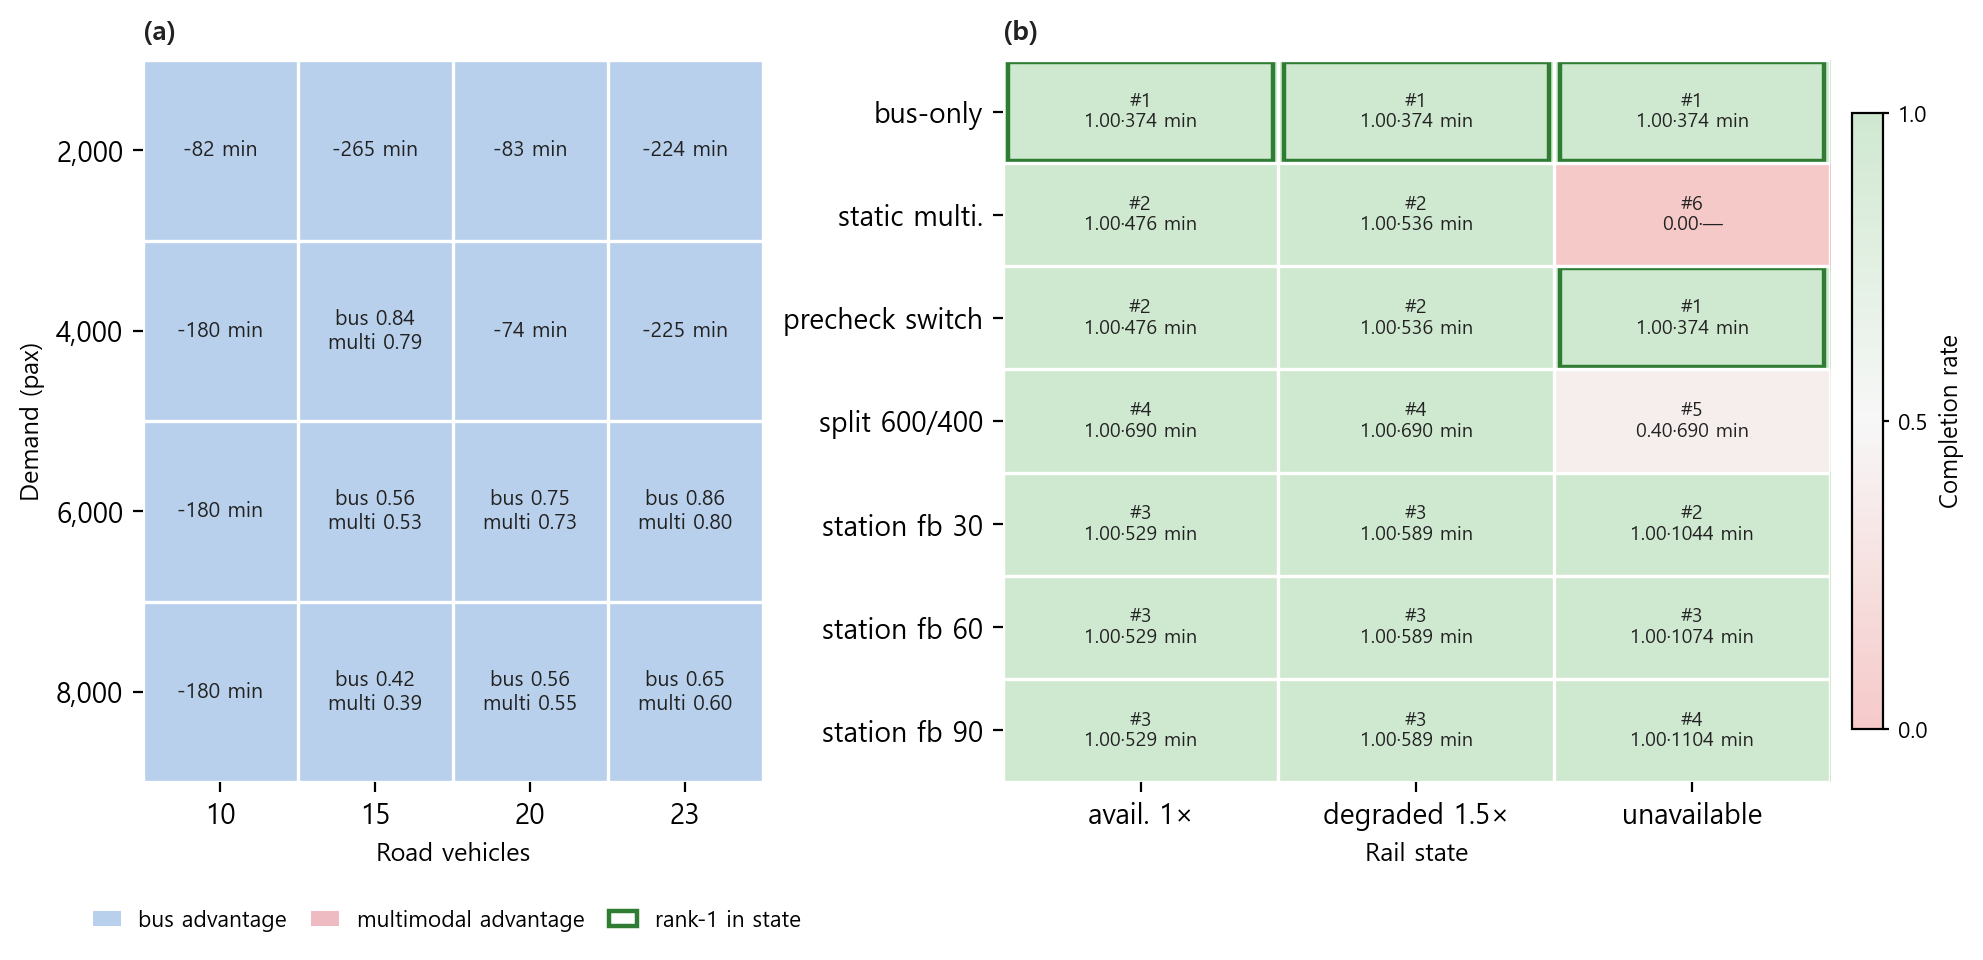
\includegraphics[width=\linewidth]{fig6.png}
\caption{Fleet scarcity and rail-state response policies (top-10, reverse empty return, 30 CRN seeds). (a) Outcome-winner map over demand (2{,}000--8{,}000 passengers) and equal total road-fleet size (10--23 vehicles) with available rail and no road damage; cell color is the lexicographic winner (blue bus-only, red multimodal, gray tie) and annotations give completion rates (bus/multi.) where they differ and mean $\Delta$ in minutes where both complete. Bus-only wins or ties every cell; higher-demand cells separate on completion rate rather than makespan. (b) Policy ranking at demand 1{,}000 and 23 road vehicles under completion-rate-then-makespan ordering; when rail is unavailable, precheck switching ties bus-only while static multimodal has completion 0.00.}
\label{fig:policies}
\end{figure}

\subsection{Rail-state response policies}
Table~\ref{tab:adaptive} ranks adaptive policies with the same lexicographic rule. Under the equal road fleet with available rail, bus-only ranks first (374.1 min); static and precheck policies take 475.8 min and split 600/400 takes 690.4 min. Under rail unavailable, static multimodal completion is 0.0; split 600/400 completion is 0.4 (rail-assigned group incomplete); precheck switching ties bus-only at 374.1 min with completion 1.0; station fallback after 30/60/90 min completes near 1{,}044/1{,}074/1{,}104 min under the equal-road-fleet frame (and near 442/472/502 min under the configured bundle). Under the configured bundle with available rail, split 600/400 ranks first (342.5 min), ahead of static/precheck/fallback (363.8) and bus-only (374.1). With rail degraded 1.5 under the configured bundle, bus-only ranks first (374.1) ahead of split (401.4) and static/precheck/fallback (423.8): partial rail degradation already removes the split advantage on this frame. All policies in this comparison use 23 road vehicles on the equal-road-fleet side (bus 23 direct; static/precheck 12 feeder + 11 last-mile; split 6 direct + 9 feeder + 8 last-mile; fallback 8 feeder + 8 last-mile + 7 reserve); rail remains additional. Rail unavailability therefore bounds a static policy, not every multimodal response design. The adaptive result is the practical hinge of the article: mode labels understate recoverable response structure.

\begin{table}[!t]
\caption{Adaptive policy means (completion rate then finite makespan; top-10, 30 seeds).}
\label{tab:adaptive}
\centering
\footnotesize
\begin{tabular}{@{}llrl@{}}
\hline
Frame / rail & Policy & Rate & Mean min \\
\hline
Conf.\ / avail. & split 600/400 & 1.00 & 342.5 \\
Conf.\ / avail. & static, precheck, fb. & 1.00 & 363.8 \\
Conf.\ / avail. & bus-only & 1.00 & 374.1 \\
Conf.\ / degr.\ 1.5 & bus-only & 1.00 & 374.1 \\
Conf.\ / degr.\ 1.5 & split 600/400 & 1.00 & 401.4 \\
Conf.\ / degr.\ 1.5 & static, precheck, fb. & 1.00 & 423.8 \\
Conf.\ / unavail. & bus-only, precheck & 1.00 & 374.1 \\
Conf.\ / unavail. & fallback 30/60/90 & 1.00 & 442/472/502 \\
Conf.\ / unavail. & split 600/400 & 0.40 & 246.1$^{a}$ \\
Conf.\ / unavail. & static multimodal & 0.00 & --- \\
Equal / avail. & bus-only & 1.00 & 374.1 \\
Equal / avail. & static, precheck & 1.00 & 475.8 \\
Equal / avail. & split 600/400 & 1.00 & 690.4 \\
Equal / unavail. & bus-only, precheck & 1.00 & 374.1 \\
Equal / unavail. & fallback 30/60/90 & 1.00 & 1044/1074/1104 \\
Equal / unavail. & split 600/400 & 0.40 & 690.4$^{a}$ \\
Equal / unavail. & static multimodal & 0.00 & --- \\
\hline
\end{tabular}
\\
$^{a}$Mean over finite incomplete-run times; not used for full-completion ranking.
\end{table}

\subsection{Random threat-set uncertainty}
Across 100 random eight-edge threat sets and 30 arrival seeds per set, all 3{,}000 configured-bundle pairs complete for both alternatives. Mean $\Delta$ is $+11.674$ min. The nested two-level interval $[9.221,\ 14.257]$ excludes zero, but it resamples arrival seeds independently inside each resampled threat draw even though the same 30 seeds are reused across all 100 draws; that dependence violation understates uncertainty. The crossed two-way interval $[-11.132,\ 32.784]$, which resamples the seed index set globally once per replicate, includes zero. The configured-bundle mean difference therefore remains \emph{unresolved} once the crossed design is respected: threat-location averaging does not separate a $+11.7$ min mean at the observed cross-threat variance, and the earlier ``resolved'' reading is withdrawn as a dependence-assumption artifact. Completion frequencies of 1.0 are empirical frequencies among generated draws, not estimates of real-event probabilities; the stored probability-proxy columns explicitly label this scope as \texttt{empirical\_\allowbreak result\_\allowbreak frequency\_\allowbreak among\_\allowbreak paired\_\allowbreak valid\_\allowbreak simulation\_\allowbreak results\_\allowbreak ... \_not\_\allowbreak event\_\allowbreak probability}. The random-threat result is therefore consistent with the fixed-scenario configured-bundle story---a small multimodal-favoring point estimate under the doubled bundle that thirty seeds cannot separate---rather than a tighter revision of it.
\subsection{Screening and replication diagnostics}
Morris trajectories screen six factors (demand, arrival sigma, rail multiplier, road fleet, transfer time, long-haul road multiplier) on \emph{completion rate}, with seven points per six-factor trajectory (base plus one step per factor), 20 trajectories, 5 arrival seeds, and 2 policies for 1{,}400 runs. Table~\ref{tab:morris} reports the elementary-effect means. For bus-only completion rate, $\mu^{*}$ ranks demand 0.533, road fleet 0.241, and long-haul multiplier 0.188; rail, transfer, and arrival sigma are 0 on the configured-bundle completion-rate scale. For static multimodal completion rate all six $\mu^{*}$ values are 0 or near 0 (ceiling at 1.0 under the tested configured-bundle ranges), with road fleet at 0.009. The bus-only ranking is consistent with the scale and demand--fleet tables: demand and fleet size are the factors that actually move completion below 1.0 inside the window, while rail and transfer parameters do not bind until a multimodal itinerary is forced past an unavailable rail leg---a state outside this configured-bundle available-rail screening range. Morris \emph{makespan} elementary effects are \emph{not} reported for this top-10 campaign: bus-only has 59 incomplete groups and 294 nonfinite seed outcomes and static multimodal has 1 incomplete group and 5 nonfinite outcomes, so the all-seed finite-makespan screening scope is incomplete by design. Completion-rate screening answers a different response question and is retained as such; no screening statistic is reported as a calibrated sensitivity product.

\begin{table}[!t]
\caption{Morris elementary effects on completion rate ($\mu^{*}$; 20 trajectories, configured bundle, available range).}
\label{tab:morris}
\centering
\footnotesize
\begin{tabular}{@{}lrr@{}}
\hline
Factor & Bus-only $\mu^{*}$ & Multi.\ $\mu^{*}$ \\
\hline
demand & 0.533 & 0.000 \\
road fleet total & 0.241 & 0.009 \\
long-haul road multiplier & 0.188 & 0.000 \\
rail multiplier & 0.000 & 0.000 \\
transfer time & 0.000 & 0.000 \\
arrival sigma & 0.000 & 0.000 \\
\hline
\end{tabular}
\\
\footnotesize{Makespan $\mu^{*}$ withheld (incomplete replication groups).}
\end{table}

At 30 baseline replications, paired-$t$ half-width is 22.88 min for the configured bundle and 23.35 min for the equal-road-fleet no-disruption cell. Half-widths shrink from 5 to 10 to 20 to 30 runs but remain wide relative to the $+10$ min configured-bundle point estimate; thirty runs are fixed for this design and do not establish universal adequacy. Supporting half-width sequences for selected configured-bundle scenarios appear in the Appendix (Table~\ref{tab:replicate}). The practical implication for readers who wish to re-run a subset of cells: if the decision of interest hinges on a mean difference smaller than roughly 20--25 min under the configured bundle, thirty paired seeds are insufficient to resolve it, and either more seeds, a narrower scenario set, or an explicit acceptance of the unresolved interval is required. Equal-road-fleet gaps of about 100 min clear this half-width comfortably, which is why the equal-road-fleet baseline is reported as resolved while the configured-bundle baseline is not.

\subsection{Path interdiction stress}
The path-interdiction campaign removes budget-$k\in\{3,5\}$ edges on the A--D shortest path under static full-horizon recovery and multiplies long-haul road time by 1.0--3.0. All 2{,}400 runs (both $k$, ten road multipliers, both frames, two policies, 30 seeds) record completion rate 0.0 for both alternatives; no finite makespan is available. Table~\ref{tab:path} summarizes the outcome pattern. Post-hoc connectivity analysis on the top-10 envelope shows the interdicted sets form a literal forward cut: after removing the interdicted edges (edge sets verified by checksum against the campaign rows), forward A$\rightarrow$D, A$\rightarrow$S, and R$\rightarrow$D are all disconnected for both $k=3$ and $k=5$, while the reverse legs retain their normal free-flow times (129.2/15.1/61.4 min). Zero completion is therefore topological disconnection of the reduced envelope under the recovery assumption, not horizon-induced noncompletion. This is a graph-scope-sensitive stress product. It is not used to re-estimate the break-even multiplier, not compared against the fixed-scenario critical-link or random-blockage cells (which do complete), and not generalized to the full national graph. The uniformity of the zero-completion outcome across both $k$ values, both frames, and the full road-multiplier ladder is itself informative: within this envelope the interdicted set disconnects rather than merely costs, so road-multiplier variation cannot rescue delivery once the cut is in place.

\begin{table}[!t]
\caption{Path-interdiction outcome summary (top-10; all cells: bus and multimodal completion 0.00).}
\label{tab:path}
\centering
\footnotesize
\begin{tabular}{@{}llcc@{}}
\hline
Budget $k$ & Road multipliers & Frames & Rows ($\Delta$ complete) \\
\hline
3 & 1.0--3.0 (10 pts) & configured, equal & 1{,}200 (0) \\
5 & 1.0--3.0 (10 pts) & configured, equal & 1{,}200 (0) \\
\hline
\end{tabular}
\end{table}

\subsection{Second corridor: protocol transferability}
The reporting protocol was re-applied to a second public-data corridor sharing the same assembly/rail anchors and national road cache but a different destination: Songpa--Yangyang (D at the Yangyang county-office centroid, with a longer last-mile leg). Corridor envelopes (626/1{,}262 top-3, 2{,}040/4{,}124 top-5, 7{,}916/16{,}126 top-10) were rebuilt from the same cache, scenarios frozen on the corridor-2 top-3 graph, and a reduced protocol run (graph audit, frame baselines, allocation surface, break-even sweep; 2{,}590 runs). Table~\ref{tab:corridor2} shows the protocol reproduces its diagnostics with different numbers. Graph-scope agreement repeats the Goseong pattern almost exactly: top-3 connectivity/ranking agreement 0.800/0.714, top-5 and top-10 at 1.000/1.000. The frame comparison does \emph{not} repeat the Goseong sign flip: on Yangyang, bus-only is resolved faster in \emph{both} frames (configured $-27.5$ $[-43.3,\ -11.8]$, equal-fleet $-49.3$ $[-65.4,\ -33.2]$), because the longer last-mile leg penalizes the multimodal itinerary under both counting rules. The best feasible split differs (8 feeder + 15 last-mile at 342.6 min versus 6/17 on Goseong), and the break-even crossing at that split is 1.278---inside the Goseong robust band's neighborhood but a different number. Transferability therefore holds for the protocol (audit thresholds, frame separation, allocation-conditional band) and not for the numerical boundary values, which are corridor-specific as the thesis requires.

\begin{table}[!t]
\caption{Second-corridor (Songpa--Yangyang) protocol outcomes versus Goseong.}
\label{tab:corridor2}
\centering
\footnotesize
\begin{tabular}{@{}lrr@{}}
\hline
Diagnostic & Goseong & Yangyang \\
\hline
Top-3 connectivity / ranking & 0.786 / 0.686 & 0.800 / 0.714 \\
Top-5 / top-10 agreement & 1.000 / 1.000 & 1.000 / 1.000 \\
Configured $\Delta$ (resolved?) & $+10.3$ (no) & $-27.5$ (yes) \\
Equal-fleet $\Delta$ at 12/11 & $-101.7$ & $-49.3$ \\
Best feasible split & 6/17 (394.6) & 8/15 (342.6) \\
Crossing at best split & 1.150 & 1.278 \\
\hline
\end{tabular}
\end{table}

\section{Discussion}
\label{sec:discussion}
Six bounded statements follow from the experiments.

First, resource definition can reverse the baseline interpretation. Configured bundles nearly tie (unresolved $+10$ min), whereas equal road fleets with the fixed 12/11 split favor bus-only by about 102 min while still granting multimodal an unmatched rail resource. Any modal claim that suppresses the frame is uninterpretable. The equal-fleet number itself is allocation-conditional: the 22-split surface runs from $-20.5$ min (unresolved) at the best 6/17 split to $-1{,}010$ min at the degenerate 22/1 split, so even holding the frame fixed, the baseline gap spans almost two orders of magnitude across feasible allocations. This is a reporting-protocol result before it is a transport result: the same simulator, seeds, and disruption set produce opposite directional stories under two reasonable counting rules, and different gaps under different splits of one rule. Tables~\ref{tab:stress} and~\ref{tab:stressconf} make the reversal visible across the full stress ladder, not only at the no-disruption baseline; empty-return KPIs in Table~\ref{tab:empties} show why the equal-road-fleet gap is a fleet-parity effect rather than a passenger-leg artifact. A reader who encounters only one frame---for example, a configured-bundle table that omits road-vehicle totals---cannot reconstruct why another study of the same corridor reached the opposite sign.

Second, under equal total road fleets and normally available rail, the mean ordering crosses near a 1.15--1.28 long-haul road multiplier for robust feeder splits (joint-seed intervals roughly 1.02--1.50), while the fixed 12/11 split crosses near 1.742 (joint-seed interval 1.550--2.003; fine grid brackets the sign change between 1.74 and 1.75). Full-graph validation reproduces both crossings (1.761 $[1.555,\ 1.989]$ and 1.150 $[1.106,\ 1.389]$), so the boundary is not a reduced-envelope artifact. The configured-bundle curve does not cross on 1.0--3.0, so no crossing is frame-free, let alone allocation-free. The boundary is decision-relevant only when a planner already accepts the equal-road-fleet frame, a stated fleet split, the top-10 envelope (or the validated full graph), normally available rail, demand 1{,}000, and the 24-h window. Outside that acceptance set---for example under configured bundles or under degraded rail---the same campaigns report a different (or unresolved) ordering and the crossing language must not be transplanted.

Third, under the equal-road-fleet frame, rail-unavailable failure belongs to static multimodal without a fallback rule; precheck switching completes at the bus-only time. Adaptive structure therefore matters as much as mode labels. Under the configured bundle, split 600/400 can even beat bus-only when rail is available (342.5 versus 374.1 min), which shows that the configured-bundle multimodal advantage is partly a response-design effect rather than an inherent rail effect; with rail degraded 1.5 that split advantage already disappears and bus-only ranks first. Rail unavailability is therefore a bound on static multimodal, not on every multimodal itinerary that can reassign passengers before departure. Fallback policies that wait 30, 60, or 90 min before switching recover completion but at a makespan cost that grows with the wait (442/472/502 min configured; 1044/1074/1104 min equal-road-fleet under unavailable rail), so precheck---which detects the outage before departure rather than after a wait---dominates the other adaptive designs whenever the outage is observable at planning time. Split 600/400 under unavailable rail leaves only the road half of the cohort deliverable (completion 0.40), which the outcome rule refuses to rank against a full-completion bus-only run.

Fourth, in the configured-bundle graph-scope check, top-5 and top-10 preserve tested connectivity and ranking while top-3 does not, and extreme long-haul slowdown grows top-10/full divergence (ratio 1.157 at 3.0). Functional-segment normal times show the mechanism: A$\rightarrow$D, A$\rightarrow$S, and R$\rightarrow$D match across scopes, while only S$\rightarrow$R separates (1.218$\times$ for top-3). Reduced graphs must be audited, not assumed, and normal-time agreement on the easy legs is not evidence of stress-set agreement on the hard leg. The audit protocol---connectivity agreement, policy-ranking agreement, and segment-time ratios against a full reference---transferred to a second corridor with the same thresholds (top-3 failing, top-5/top-10 at full agreement), even though every numerical boundary value differed there.

Fifth, demand and fleet pressure change the response question. At demand 2{,}000 both frames complete and the frame split remains; at demand 6{,}000--12{,}000 at the break-even road multiplier, configured-bundle bus completion falls to about 0.86--0.43 while multimodal holds 1.00 through 8{,}000. Those cells are completion-stress outcomes under a fixed 24-h window, not makespan comparisons. The asymmetry follows from itinerary structure rather than from an intrinsic scalability property: once demand exceeds what 23 direct buses can deliver inside 1{,}440 min, bus-only completion drops, while multimodal still has the configured 46-road-vehicle bundle plus rail headway capacity. At 12{,}000 even configured multimodal falls to 0.81, so the window eventually saturates both alternatives; language beyond that point is again completion-rate language only. Morris screening ranks demand first for bus-only completion rate ($\mu^{*}=0.533$), consistent with the scale table, but no screening statistic is presented as a calibrated sensitivity product and makespan elementary effects are withheld for incomplete replication groups.

Sixth, blocked roads reroute, but explicit path interdiction does not. Critical-link and fixed random-blockage scenarios complete for both alternatives and do not support a collapse narrative on this envelope. By contrast, budget-$k$ path interdiction under blocked-edge recovery yields zero completion for both alternatives in all 2{,}400 path-interdiction runs on the top-10 graph (both $k$, all road multipliers, both frames, demand 1{,}000). Post-hoc connectivity analysis confirms the interdicted sets form a literal forward cut of the envelope (forward A$\rightarrow$D, A$\rightarrow$S, R$\rightarrow$D disconnected; reverse legs at normal times) under static full-horizon recovery; it is a graph-scope-sensitive stress result and is not used to re-estimate the break-even multiplier. The contrast between completing blockage cells and non-completing interdiction cells is itself a design lesson: ``link removed'' is not a single treatment---selection rule (betweenness versus shortest-path budget-$k$), recovery assumption, and envelope all matter.

Two additional readings keep the results inside the claim boundary. (i) The configured-bundle random-threat crossed interval $[-11.13,\ 32.78]$ is a crossed-design interval over generated threats; it does not convert simulation frequency into event probability, and it leaves the small configured-bundle mean unresolved. (ii) Demand--fleet completion separation at 4{,}000--8{,}000 is a capacity-window phenomenon: when only one alternative finishes, makespan language is withheld by the outcome rule.

It would be incorrect to read these results as proof that one mode is superior under all conditions. The strongest portable claim is conditional: under stated corridor, graph, resource, rail, window, and policy conditions, average completion-time ordering behaves as reported. Practitioners should therefore require five disclosures---resource frame, fleet allocation, graph scope, rail state, and response rule---before accepting any bus-versus-multimodal ranking in comparable wartime planning studies. Empty-return KPIs and replicate-count half-widths are recommended as two further disclosures whenever finite fleets and small mean differences are in play.

A second reading error to avoid is treating the break-even multiplier as a corridor-invariant physical constant. The robust-split crossings near 1.15--1.28 are interpolated properties of mean $\Delta$ on one top-10 envelope, one demand level, one fleet profile, one allocation band, and one rail-availability state; the joint-seed bootstrap intervals alone span several tenths of multiplier units, the fixed-12/11 crossing sits far higher at 1.742, and the configured-bundle curve does not cross at all on the tested 1.0--3.0 range. Reporting any crossing without its acceptance set would reproduce exactly the kind of frame-suppressed modal claim this article argues against. The same discipline applies to the adaptive-policy rankings: precheck, split, and fallback advantages are stated against a named rail condition and a named resource frame, never as free-standing policy orderings.

\section{Limitations and Claim Boundaries}
\label{sec:limits}
This work is a public-data-based conditional scenario simulation for decision support. It is not a field-use movement plan. Formal study flags remain false by design; human review is required before any stronger claim. Specific limitations include the following.

\emph{Scope and data.} The study uses two public-data case corridors (Songpa--Goseong and Songpa--Yangyang) sharing one national road cache, with public administrative and station coordinates only; results do not transfer to other corridors without a new graph-scope audit, and the two corridors already disagree on frame-level rankings. Charter-rail runtime, low background traffic (100 veh/h), fleet role sizes, demand fixture scale, and threat generation are planning assumptions or sensitivity fixtures, not calibrated wartime measurements. Per-class road speeds and capacities follow public manuals and observed tag medians; they are not fitted to wartime traffic observations, which do not exist in public form.

\emph{Resource accounting.} Equal road-vehicle count is not equal cost: rail capacity, energy, crew, and monetary cost remain unmatched. Configured-bundle multimodal uses 46 road vehicles against bus-only's 23; equal-road-fleet multimodal still receives rail as an additional resource. Neither frame is an equal-expenditure comparison, and within the equal-road-fleet frame the ranking further depends on the feeder/last-mile split, which must be disclosed alongside the frame.

\emph{Graph and adversarial scope.} Top-10 diverges from full scope under extreme long-haul slowdown (ratio 1.157 at 3.0). Random threat sets are generated stress samples, not an empirical threat distribution. Path-interdiction zero-completion outcomes are envelope-specific under static full-horizon recovery and are not full-graph proofs; a full-graph interdiction rerun is left open. Critical-link and random-blockage completion shows only that those selection rules do not cut this envelope.

\emph{Inference and window.} Thirty paired replications leave wide half-widths (about 23 min at $n{=}30$ for baseline cells), so small configured-bundle differences are reported as unresolved rather than as zero. Replicate-count tables prevent a blanket adequacy claim. The 24-h window saturates completion on part of the demand--fleet grid, after which makespan language is withheld. Morris makespan screening is withheld for incomplete top-10 replication scopes; completion-rate screening is retained and is not a calibration product. Simulation frequencies are not event probabilities.

\emph{Omitted mechanisms.} Station processing limits, train acquisition under contingency, crew constraints, driver hours, monetary cost, passenger mode choice, and dynamic recovery inside the window are omitted. Transfer and assembly wait are logged but not optimized. Reverse empty legs are simulated on the current disrupted graph but do not consume fuel or crew hours as separate resources; only trip counts and minutes are reported for empties. Road traffic following the 100 veh/h planning input does not generate endogenous queue spillback at intersections; link performance is the rolling-window BPR term alone, which is inert at that volume relative to class capacity.

\emph{Reproducibility boundary.} The reported products are regenerable from the committed design manifest, scenario table, road-class override table, and GraphML cache identified by SHA-256. Absolute floating-point reproducibility across BLAS and NetworkX versions is not claimed beyond the pinned environment used for the paper campaigns; seed blocks and bootstrap seeds are fixed so that a re-run inside that environment is expected to match. Third-party readers who rebuild the cache from the public shapefile should verify the committed graph hash before comparing campaign rows.

Claims of the form ``field-verified,'' ``empirically fitted,'' ``predictive,'' ``live,'' ``best route,'' ``operational plan,'' ``forecast,'' ``calibrated,'' ``validated,'' ``final-ready,'' or ``ready for field use'' are outside the evidence boundary of this study. The reserved claim guard audits the manuscript for these terms and for related readiness language.

\section{Conclusion}
\label{sec:conclusion}
This study turns a modal-ranking question into a conditional boundary problem. Graph-scope auditing removes unsupported top-3 disconnection claims; physical empty returns make fleet scarcity active and observable in KPIs; resource-frame separation exposes the role of unequal bundles; paired, bootstrap, joint-seed, and crossed two-way inference separate arrival and threat-set variation without overstating what threat averaging resolves; replicate-count half-widths bound what thirty runs can resolve; and adaptive policies distinguish static rail dependence from recoverable response designs.

Under equal total road fleets and normally available rail in this case corridor, average completion-time ordering changes near a 1.15--1.28 long-haul road multiplier for robust feeder splits (1.742 for the fixed 12/11 split), each with its joint-seed uncertainty interval; fine grids bracket each sign change between adjacent grid points. Under configured bundles the baseline difference is unresolved and no crossing appears on 1.0--3.0. When rail is unavailable, only static multimodal fails while precheck switching recovers bus-level completion; under available rail, split 600/400 can beat bus-only on the configured frame. Demand scaling shows configured-bundle bus completion falling faster than multimodal once the window saturates, and budget-$k$ path interdiction on the reduced envelope fails both alternatives in every tested cell---a scope-limited stress result, not a break-even input.

Taken together, the campaigns show that a wartime bus-versus-multimodal comparison is under-specified until resource frame, graph scope, rail state, response policy, and inference product are named. The simulator and campaign design used here make each of those dimensions explicit and separately reportable; the resulting boundaries are corridor-conditional decision support rather than mode rankings. The reporting protocol---declare the frame, audit the graph, separate rail states, disclose empty-return and replicate diagnostics, and scope adversarial stresses---is the transferable contribution.

Every reuse of these boundaries must retain corridor, graph, resource, rail, time-window, and policy conditions. The methodological package---resource frames, reverse-network empty return, explicit rail states, reduced-graph audit, separated inference products, and an explicit path-interdiction scope rule---is offered as a reporting protocol for conditional wartime transport simulation, not as a general ranking of modes. Future work that can relax current limits includes full-graph path-interdiction reruns, equal-cost resource accounting, station-processing constraints, and multi-window recovery dynamics.

For a planner reading only the headline numbers, the operational takeaway is conditional rather than modal. Configured-bundle multimodal and bus-only remain statistically unresolved under normally available rail with equal arrival seeds; equalizing total road fleets makes bus-only faster on completion time against badly split multimodal fleets and statistically tied against well-split ones, while still granting the multimodal alternative an unmatched rail leg; and long-haul road damage changes that ordering only past a corridor- and allocation-specific slowdown boundary (near 1.15--1.28 for robust splits, near 1.74 for the fixed 12/11 policy) whose uncertainty band remains wide enough that a single point estimate should not be quoted without its interval. Rail unavailability is the state in which static multimodal fails outright, and the adaptive precheck policy is the response design that restores bus-level completion under that state. Demand growth degrades the configured-bundle bus alternative first, because the direct-road itinerary saturates the 24-h window before the feeder--rail--last-mile itinerary does; that asymmetry is a completion-rate statement under a fixed window, not a claim that multimodal infrastructure is intrinsically more scalable beyond this corridor and fleet.

\section*{Code and Data Availability}
The simulation engine, experiment design manifest, campaign outputs, and analysis tables that support this article are available in the project repository at
\underline{https://github.com/\allowbreak hyunjun1121/\allowbreak transport-system-sim}
and in the versioned archival deposit on Zenodo at
\underline{https://doi.\allowbreak org/\allowbreak 10.5281/\allowbreak zenodo.\allowbreak 22953096}.
The archived bundle is version \texttt{paper-revision-\allowbreak top10-\allowbreak v4-\allowbreak 20260925-\allowbreak datacode} under the MIT License.
Road-network geometry is regenerable from the public Standard Node-Link shapefile via the committed cache-build scripts; the large GraphML cache itself is intentionally excluded from the repository and is identified by a committed SHA-256 manifest. No live external network calls are required on the default run path. Inputs carry explicit source classes (public, literature-derived, sensitivity-only, scenario-based) in the design and parameter tables. Analysis CSVs referenced in Section~VI (paired summary, break-even coarse and fine, road--rail map, demand--fleet, scale, adaptive policies, Morris effects, replicate convergence, graph-scope agreement, random-threat hierarchical and crossed two-way bootstraps, corridor-target scope metrics, path-interdiction inventory, allocation surface, full-graph break-even, break-even sensitivity, second-corridor results, and compute frontier) ship with the archival deposit.

\appendices

\section{Supporting Tables}
\label{app:tables}
This appendix collects diagnostics that support Section~VI but do not enter the main page budget. Table~\ref{tab:replicate} reports paired-$t$ half-widths at 5/10/20/30 replications for selected configured-bundle scenarios; half-widths remain on the order of tens of minutes at 30 runs, which is why small configured-bundle differences are reported as unresolved rather than as zero. Table~\ref{tab:fullroad} lists the full available-rail equal-road-fleet road--rail mean $\Delta$ series used to construct the coarse break-even crossing, including the 1.6/1.8 bracket. Table~\ref{tab:scopelegs} repeats the functional-segment detour ratios against the full reference so that the top-3 S$\rightarrow$R 1.218 figure and the top-10 1.015 figure are visible together with the exact-match legs.

\begin{table}[!t]
\caption{Paired-$t$ half-width (min) by replicate count for selected configured-bundle no-disruption and stress cells (top-10).}
\label{tab:replicate}
\centering
\footnotesize
\begin{tabular}{@{}lrrrr@{}}
\hline
Scenario & $n{=}5$ & $n{=}10$ & $n{=}20$ & $n{=}30$ \\
\hline
No disruption & 79.2 & 41.1 & 25.0 & 22.9 \\
Access severe & 83.6 & 43.6 & 25.9 & 23.7 \\
Last-mile severe & 84.4 & 45.9 & 26.0 & 23.8 \\
Long-haul mild & 87.8 & 45.6 & 27.4 & 25.2 \\
Long-haul moderate & 100.6 & 52.4 & 31.1 & 28.8 \\
Long-haul severe & 164.6 & 86.9 & 50.0 & 45.4 \\
\hline
\end{tabular}
\end{table}

\begin{table}[!t]
\caption{Fixed-12/11-split available-rail mean $\Delta$ (bus $-$ multi., min) by long-haul road multiplier (top-10, 30 seeds; coarse break-even series).}
\label{tab:fullroad}
\centering
\footnotesize
\begin{tabular}{@{}rr@{\qquad}rr@{}}
\hline
Road mult. & Mean $\Delta$ & Road mult. & Mean $\Delta$ \\
\hline
1.00 & $-101.71$ & 1.40 & $-46.90$ \\
1.10 & $-88.00$ & 1.425 & $-43.47$ \\
1.20 & $-74.30$ & 1.45 & $-40.05$ \\
1.25 & $-67.45$ & 1.475 & $-36.62$ \\
1.30 & $-60.60$ & 1.50 & $-33.19$ \\
1.35 & $-53.75$ & 1.60 & $-19.49$ \\
 & & 1.80 & $+7.91$ \\
 & & 2.00 & $+35.45$ \\
 & & 2.50 & $+104.74$ \\
 & & 3.00 & $+173.69$ \\
\hline
\end{tabular}
\end{table}

\begin{table}[!t]
\caption{Functional-segment travel-time detour ratio versus full reference (normal free-flow).}
\label{tab:scopelegs}
\centering
\footnotesize
\begin{tabular}{@{}lrrrr@{}}
\hline
Scope & A$\rightarrow$D & A$\rightarrow$S & R$\rightarrow$D & S$\rightarrow$R \\
\hline
top-3 & 1.000 & 1.000 & 1.000 & 1.218 \\
top-5 & 1.000 & 1.000 & 1.000 & 1.040 \\
top-10 & 1.000 & 1.000 & 1.000 & 1.015 \\
\hline
\end{tabular}
\end{table}

Additional campaign inventory, full road--rail map cells, and the complete adaptive-policy grid are stored with the analysis CSVs referenced in Section~X. Those files retain per-scenario completion counts, excluded-pair reasons, and bootstrap seeds (bootstrap seed 20260721 throughout).

\begin{thebibliography}{00}

\bibitem{b1} H. Jin, S. Park, and C. Suh, ``A study on wartime multimodal transportation decision-making using simulation,'' \emph{J. Korea Soc. Comput. Appl.}, vol. 23, no. 4, pp. 252--258, 2022, doi: 10.5762/KAIS.2022.23.4.252.

\bibitem{b2} Ministry of Land, Infrastructure and Transport and Korea Transport Institute, \emph{2013 Highway Capacity Manual} (Doro Yongnyang Pyoram). Sejong, South Korea: MOLIT/KOTI, 2013.

\bibitem{b3} Enforcement Rules of the Road Traffic Act, Art.~19 (Speed of Motor Vehicles, etc.), National Law Information Center, Seoul, South Korea [Online]. Available: \underline{https://www.law.go.kr}

\bibitem{b4} M. G. H. Bell, ``A game theory approach to measuring the performance reliability of transport networks,'' \emph{Transp. Res. Part B Methodol.}, vol. 34, no. 6, pp. 533--545, 2000, doi: 10.1016/S0191-2615(99)00042-9.

\bibitem{b5} Bureau of Public Roads, \emph{Traffic Assignment Manual for Application with a Large, High Speed Computer}. Washington, DC, USA: U.S. Dept. Commerce, 1964.

\bibitem{b6} C. F. Daganzo, ``The cell transmission model: A dynamic representation of highway traffic consistent with the hydrodynamic theory,'' \emph{Transp. Res. Part B Methodol.}, vol. 28, no. 4, pp. 269--287, 1994, doi: 10.1016/0191-2615(94)90002-7.

\bibitem{b7} T. F. Fwa, Ed., \emph{The Handbook of Highway Engineering}. Boca Raton, FL, USA: CRC Press, 2006, doi: 10.1201/9781420039504.

\bibitem{b8} A. Hagberg, D. Schult, and P. Swart, ``Exploring network structure, dynamics, and function using NetworkX,'' in \emph{Proc. SciPy}, 2008, pp. 11--15, doi: 10.25080/TCWV9851.

\bibitem{b9} C. R. Harris \emph{et al.}, ``Array programming with NumPy,'' \emph{Nature}, vol. 585, pp. 357--362, 2020, doi: 10.1038/s41586-020-2649-2.

\bibitem{b10} E. Jenelius, T. Petersen, and L.-G. Mattsson, ``Importance and exposure in road network vulnerability analysis,'' \emph{Transp. Res. Part A Policy Pract.}, vol. 40, no. 7, pp. 537--560, 2006, doi: 10.1016/j.tra.2005.11.003.

\bibitem{b11} A. M. Law, \emph{Simulation Modeling and Analysis}, 5th ed. New York, NY, USA: McGraw-Hill Education, 2014.

\bibitem{b12} M. D. Morris, ``Factorial sampling plans for preliminary computational experiments,'' \emph{Technometrics}, vol. 33, no. 2, pp. 161--174, 1991, doi: 10.1080/00401706.1991.10484804.

\bibitem{b13} P. M. Murray-Tuite, ``A framework for evaluating risk to the transportation network from terrorism and security policies,'' \emph{Int. J. Crit. Infrastruct.}, vol. 3, no. 3/4, pp. 389--407, 2007, doi: 10.1504/IJCIS.2007.014117.

\bibitem{b14} A. Nicholson and Z.-P. Du, ``Degradable transportation systems: An integrated equilibrium model,'' \emph{Transp. Res. Part B Methodol.}, vol. 31, no. 3, pp. 209--223, 1997, doi: 10.1016/S0191-2615(96)00022-7.

\bibitem{b15} D. M. Scott, D. C. Novak, L. Aultman-Hall, and F. Guo, ``Network robustness index: A new method for identifying critical links and evaluating the performance of transportation networks,'' \emph{J. Transport Geogr.}, vol. 14, no. 3, pp. 215--227, 2006, doi: 10.1016/j.jtrangeo.2005.10.003.

\bibitem{b16} Y. Sheffi, \emph{Urban Transportation Networks: Equilibrium Analysis with Mathematical Programming Methods}. Englewood Cliffs, NJ, USA: Prentice-Hall, 1985.

\bibitem{b17} Ministry of Land, Infrastructure and Transport, Standard Node-Link (pyojun node-link), National Transport Information Center (NTIS), Seoul, South Korea [Online]. Available: \underline{https://www.its.go.kr}

\bibitem{b18} KORAIL, Gangneung Line KTX-Eum timetable, Seoul, South Korea [Online]. Available: \underline{https://www.korail.com} (accessed: 2026-07-18).

\bibitem{b19} L. Mattsson and E. Jenelius, ``Vulnerability and resilience of transport systems---A discussion of recent research,'' \emph{Transp. Res. Part A Policy Pract.}, vol. 81, pp. 1--18, 2015, doi: 10.1016/j.tra.2015.06.002.

\bibitem{b20} M. G. H. Bell and H. Iida, \emph{Transportation Network Analysis}. Chichester, U.K.: Wiley, 1997.

\bibitem{b21} R. K. Ahuja, T. L. Magnanti, and J. B. Orlin, \emph{Network Flows: Theory, Algorithms, and Applications}. Englewood Cliffs, NJ, USA: Prentice-Hall, 1993.

\bibitem{b22} A. Saltelli, S. Tarantola, F. Campolongo, and T. Ratto, \emph{Sensitivity Analysis: A Guide to Scientific Assessment}. Hoboken, NJ, USA: Wiley, 2008.

\bibitem{b23} J. Kleijnen, \emph{Design and Analysis of Simulation Experiments}, 2nd ed. Cham, Switzerland: Springer, 2015.

\bibitem{b24} K. G. Murty, \emph{Network Programming: Algorithms, Models and Applications for Road, Rail, Air and Water Transportation}. Hoboken, NJ, USA: Wiley, 2022.

\bibitem{b25} E. W. Dijkstra, ``A note on two problems in connexion with graphs,'' \emph{Numer. Math.}, vol. 1, pp. 269--271, 1959, doi: 10.1007/BF01386390.

\bibitem{b26} J. Yen, ``Finding the shortest loopless paths in a network,'' \emph{Manage. Sci.}, vol. 17, no. 11, pp. 712--716, 1971, doi: 10.1287/mnsc.17.11.712.

\bibitem{b27} T. H. Cormen, C. E. Leiserson, R. L. Rivest, and C. Stein, \emph{Introduction to Algorithms}, 4th ed. Cambridge, MA, USA: MIT Press, 2022.

\bibitem{b28} E. Israeli and R. K. Wood, ``Shortest-path network interdiction,'' \emph{Networks}, vol. 40, no. 2, pp. 97--111, 2002, doi: 10.1002/net.10047.

\bibitem{b29} D. W. Smith and H. N. Song, ``A survey of network interdiction models and methods,'' \emph{Eur. J. Oper. Res.}, vol. 276, no. 2, pp. 395--411, 2019, doi: 10.1016/j.ejor.2019.01.014.

\bibitem{b30} National Transport Information Center, Public Data Portal road-network file metadata, Seoul, South Korea [Online]. Available: \underline{https://www.data.go.kr}

\bibitem{b31} B. Chen, S. Hu, X. Xu, G. Wang, D.-H. Lee, and Z. He, ``A survey of multi-modal urban transportation network resilience: modeling, evaluation, and optimization,'' \emph{Transp. Res. Part E Logist. Transp. Rev.}, vol. 207, Art. no. 104634, 2026, doi: 10.1016/j.tre.2025.104634.

\bibitem{b32} A. S. Bergantino, A. Gardelli, and L. Rotaris, ``Assessing transport network resilience: empirical insights from real-world data studies,'' \emph{Transp. Rev.}, vol. 44, no. 4, pp. 834--857, 2024, doi: 10.1080/01441647.2024.2322434.

\bibitem{b33} W. Ma, S. Lin, Y. Ci, and R. Li, ``Resilience evaluation and improvement of post-disaster multimodal transportation networks,'' \emph{Transp. Res. Part A Policy Pract.}, vol. 189, Art. no. 104243, 2024, doi: 10.1016/j.tra.2024.104243.

\bibitem{b34} K. Qu, X. Fan, X. Xu, G. A. Hanasusanto, and A. Chen, ``Improving transportation network redundancy under uncertain disruptions via retrofitting critical components,'' \emph{Transp. Res. Part B Methodol.}, vol. 194, Art. no. 103174, 2025, doi: 10.1016/j.trb.2025.103174.

\bibitem{b35} C. A. Iliopoulou, M. Makridis, and A. Kouvelas, ``Improving transit network resilience against disruptions through path redundancy,'' \emph{Socio-Econ. Plan. Sci.}, vol. 100, Art. no. 102228, 2025, doi: 10.1016/j.seps.2025.102228.

\end{thebibliography}

\begin{IEEEbiographynophoto}{Hyunjun Kim}
Hyunjun Kim is currently pursuing the B.S. degree in computer science at the Korea Advanced Institute of Science and Technology (KAIST), Daejeon, Republic of Korea. He is currently an AI Researcher with the Korea Military Academy (KMA), Seoul, Republic of Korea. His research lies at the intersection of large language models, AI safety, and trustworthy AI, including retrieval-augmented generation, reliable evaluation methodologies, and autonomous AI agents. His current research interests include AI safety and security, adversarial robustness of large language models, reliable evaluation, retrieval-augmented generation, and simulation-supported decision support. His ORCID is https://orcid.org/0009-0009-5791-9468.
\end{IEEEbiographynophoto}

\begin{IEEEbiographynophoto}{Jae Woo Lee}
Jae Woo Lee received the B.S. degree, with majors in biosystems engineering and mechanical engineering and with highest honors, from Seoul National University, Seoul, Republic of Korea, in 2021. He is currently pursuing the M.S. degree in medicine at CHA University, Seongnam, Republic of Korea. From 2020 to 2021, he was a Research Intern with the ORED Laboratory, Seoul National University. Since 2024, he has been a Medical Data Analysis Researcher with the Department of Orthopedic Surgery, CHA University, and since 2025, an AI Researcher with the Korea Military Academy. He received first place and the Minister of National Defense Award at the 2025 Defense AI Competition. His research interests include clinical medicine and artificial intelligence, data-driven medical research, and interdisciplinary methods that bridge medicine and AI. His ORCID is https://orcid.org/0009-0009-8988-1513.
\end{IEEEbiographynophoto}

\begin{IEEEbiographynophoto}{Hyunho Kim}
Hyunho Kim received the Ph.D. degree from Auburn University, Auburn, AL, USA, in 2009. He is currently an Associate Professor with the Department of Economics, Korea Military Academy, Seoul, Republic of Korea. His research and teaching interests include queueing theory, simulation, optimization, and economics, with applications to transportation and logistics decision support. He can be contacted at kimhyuh@kma.ac.kr. His ORCID is https://orcid.org/0009-0007-6847-6696.
\end{IEEEbiographynophoto}

\EOD

\end{document}
